% Options for packages loaded elsewhere
% Options for packages loaded elsewhere
\PassOptionsToPackage{unicode}{hyperref}
\PassOptionsToPackage{hyphens}{url}
\PassOptionsToPackage{dvipsnames,svgnames,x11names}{xcolor}
%
\documentclass[
  single column]{article}
\usepackage{xcolor}
\usepackage[top=30mm,left=25mm,heightrounded,headsep=22pt,headheight=11pt,footskip=33pt,ignorehead,ignorefoot]{geometry}
\usepackage{amsmath,amssymb}
\setcounter{secnumdepth}{-\maxdimen} % remove section numbering
\usepackage{iftex}
\ifPDFTeX
  \usepackage[T1]{fontenc}
  \usepackage[utf8]{inputenc}
  \usepackage{textcomp} % provide euro and other symbols
\else % if luatex or xetex
  \usepackage{unicode-math} % this also loads fontspec
  \defaultfontfeatures{Scale=MatchLowercase}
  \defaultfontfeatures[\rmfamily]{Ligatures=TeX,Scale=1}
\fi
\usepackage[]{libertinus}
\ifPDFTeX\else
  % xetex/luatex font selection
\fi
% Use upquote if available, for straight quotes in verbatim environments
\IfFileExists{upquote.sty}{\usepackage{upquote}}{}
\IfFileExists{microtype.sty}{% use microtype if available
  \usepackage[]{microtype}
  \UseMicrotypeSet[protrusion]{basicmath} % disable protrusion for tt fonts
}{}
\makeatletter
\@ifundefined{KOMAClassName}{% if non-KOMA class
  \IfFileExists{parskip.sty}{%
    \usepackage{parskip}
  }{% else
    \setlength{\parindent}{0pt}
    \setlength{\parskip}{6pt plus 2pt minus 1pt}}
}{% if KOMA class
  \KOMAoptions{parskip=half}}
\makeatother
% Make \paragraph and \subparagraph free-standing
\makeatletter
\ifx\paragraph\undefined\else
  \let\oldparagraph\paragraph
  \renewcommand{\paragraph}{
    \@ifstar
      \xxxParagraphStar
      \xxxParagraphNoStar
  }
  \newcommand{\xxxParagraphStar}[1]{\oldparagraph*{#1}\mbox{}}
  \newcommand{\xxxParagraphNoStar}[1]{\oldparagraph{#1}\mbox{}}
\fi
\ifx\subparagraph\undefined\else
  \let\oldsubparagraph\subparagraph
  \renewcommand{\subparagraph}{
    \@ifstar
      \xxxSubParagraphStar
      \xxxSubParagraphNoStar
  }
  \newcommand{\xxxSubParagraphStar}[1]{\oldsubparagraph*{#1}\mbox{}}
  \newcommand{\xxxSubParagraphNoStar}[1]{\oldsubparagraph{#1}\mbox{}}
\fi
\makeatother


\usepackage{longtable,booktabs,array}
\usepackage{calc} % for calculating minipage widths
% Correct order of tables after \paragraph or \subparagraph
\usepackage{etoolbox}
\makeatletter
\patchcmd\longtable{\par}{\if@noskipsec\mbox{}\fi\par}{}{}
\makeatother
% Allow footnotes in longtable head/foot
\IfFileExists{footnotehyper.sty}{\usepackage{footnotehyper}}{\usepackage{footnote}}
\makesavenoteenv{longtable}
\usepackage{graphicx}
\makeatletter
\newsavebox\pandoc@box
\newcommand*\pandocbounded[1]{% scales image to fit in text height/width
  \sbox\pandoc@box{#1}%
  \Gscale@div\@tempa{\textheight}{\dimexpr\ht\pandoc@box+\dp\pandoc@box\relax}%
  \Gscale@div\@tempb{\linewidth}{\wd\pandoc@box}%
  \ifdim\@tempb\p@<\@tempa\p@\let\@tempa\@tempb\fi% select the smaller of both
  \ifdim\@tempa\p@<\p@\scalebox{\@tempa}{\usebox\pandoc@box}%
  \else\usebox{\pandoc@box}%
  \fi%
}
% Set default figure placement to htbp
\def\fps@figure{htbp}
\makeatother


% definitions for citeproc citations
\NewDocumentCommand\citeproctext{}{}
\NewDocumentCommand\citeproc{mm}{%
  \begingroup\def\citeproctext{#2}\cite{#1}\endgroup}
\makeatletter
 % allow citations to break across lines
 \let\@cite@ofmt\@firstofone
 % avoid brackets around text for \cite:
 \def\@biblabel#1{}
 \def\@cite#1#2{{#1\if@tempswa , #2\fi}}
\makeatother
\newlength{\cslhangindent}
\setlength{\cslhangindent}{1.5em}
\newlength{\csllabelwidth}
\setlength{\csllabelwidth}{3em}
\newenvironment{CSLReferences}[2] % #1 hanging-indent, #2 entry-spacing
 {\begin{list}{}{%
  \setlength{\itemindent}{0pt}
  \setlength{\leftmargin}{0pt}
  \setlength{\parsep}{0pt}
  % turn on hanging indent if param 1 is 1
  \ifodd #1
   \setlength{\leftmargin}{\cslhangindent}
   \setlength{\itemindent}{-1\cslhangindent}
  \fi
  % set entry spacing
  \setlength{\itemsep}{#2\baselineskip}}}
 {\end{list}}
\usepackage{calc}
\newcommand{\CSLBlock}[1]{\hfill\break\parbox[t]{\linewidth}{\strut\ignorespaces#1\strut}}
\newcommand{\CSLLeftMargin}[1]{\parbox[t]{\csllabelwidth}{\strut#1\strut}}
\newcommand{\CSLRightInline}[1]{\parbox[t]{\linewidth - \csllabelwidth}{\strut#1\strut}}
\newcommand{\CSLIndent}[1]{\hspace{\cslhangindent}#1}



\setlength{\emergencystretch}{3em} % prevent overfull lines

\providecommand{\tightlist}{%
  \setlength{\itemsep}{0pt}\setlength{\parskip}{0pt}}



 


\usepackage{booktabs}
\usepackage{longtable}
\usepackage{array}
\usepackage{multirow}
\usepackage{wrapfig}
\usepackage{float}
\usepackage{colortbl}
\usepackage{pdflscape}
\usepackage{tabu}
\usepackage{threeparttable}
\usepackage{threeparttablex}
\usepackage[normalem]{ulem}
\usepackage{makecell}
\usepackage{xcolor}
\let\oldtabular\tabular
\renewcommand{\tabular}{\small\oldtabular}
\setlength{\tabcolsep}{4pt}
\makeatletter
\@ifpackageloaded{caption}{}{\usepackage{caption}}
\AtBeginDocument{%
\ifdefined\contentsname
  \renewcommand*\contentsname{Table of contents}
\else
  \newcommand\contentsname{Table of contents}
\fi
\ifdefined\listfigurename
  \renewcommand*\listfigurename{List of Figures}
\else
  \newcommand\listfigurename{List of Figures}
\fi
\ifdefined\listtablename
  \renewcommand*\listtablename{List of Tables}
\else
  \newcommand\listtablename{List of Tables}
\fi
\ifdefined\figurename
  \renewcommand*\figurename{Figure}
\else
  \newcommand\figurename{Figure}
\fi
\ifdefined\tablename
  \renewcommand*\tablename{Table}
\else
  \newcommand\tablename{Table}
\fi
}
\@ifpackageloaded{float}{}{\usepackage{float}}
\floatstyle{ruled}
\@ifundefined{c@chapter}{\newfloat{codelisting}{h}{lop}}{\newfloat{codelisting}{h}{lop}[chapter]}
\floatname{codelisting}{Listing}
\newcommand*\listoflistings{\listof{codelisting}{List of Listings}}
\makeatother
\makeatletter
\makeatother
\makeatletter
\@ifpackageloaded{caption}{}{\usepackage{caption}}
\@ifpackageloaded{subcaption}{}{\usepackage{subcaption}}
\makeatother
\usepackage{bookmark}
\IfFileExists{xurl.sty}{\usepackage{xurl}}{} % add URL line breaks if available
\urlstyle{same}
\hypersetup{
  pdftitle={Your Title},
  pdfauthor={YOUR NAME},
  pdfkeywords={Causal
Inference, Church, Cross-validation, Distress, Health, Longitudinal, Machine
Learning, Religion, Semi-parametric, Targeted Learning},
  colorlinks=true,
  linkcolor={blue},
  filecolor={Maroon},
  citecolor={Blue},
  urlcolor={Blue},
  pdfcreator={LaTeX via pandoc}}


\title{Your Title}
\author{YOUR NAME}
\date{2025-05-12}
\begin{document}
\maketitle
\begin{abstract}
\textbf{Background}: (Brief few sentences)

\textbf{Objectives}: 1. Estimate the causal effect of YOUR EXPOSURE on
YOUR OUTCOMES measured one year later. 2. Evaluate whether these effects
vary across the population. 3. Provide policy guidance on which
individuals might benefit most.

\textbf{Method}: We conducted a three-wave retrospective cohort study
(waves XX-XXX, October XXXX--October XXXX) using data from the New
Zealand Attitudes and Values Study, a nationally representative panel.
Participants were eligible if they participated in the NZAVS in the
baseline wave (XXXX, were under the age of 62, and were employed
\textgreater{} 20 hours per week. We defined the exposure as (XXXX
\textgreater{} NUMBER on a 1-7 Likert Scale (1 = yes, 0 = no)). To
address attrition, we applied inverse probability of censoring weights;
to improve external validity, we applied weighted to the population
distribution of Age, Ethnicity, and Gender. We computed expected mean
outcomes for the population in each exposure condition (high XXXX/low
XXXXX). Under standard causal assumptions of unconfoundedness, the
contrast provides an unbiased average treatment effect. We then used
causal forests to detect heterogeneity in these effects and employed
policy tree algorithms to identify individuals (``strong responders'')
likely to experience the greatest benefits.

\textbf{Results}: Increasing XXXXX leads to XXXXX. Heterogeneous
responses to (e.g.~\emph{Forgiveness}, \emph{Personal Well-Being}, and
\emph{Life-Satisfaction}\ldots) reveal structural variability in
subpopulations\ldots{}

\textbf{Implications}: (Brief few sentences) \textbf{Keywords}:
\emph{Causal Inference}; \emph{Cross-validation}; \emph{Distress};
\emph{Employment}; \emph{Longitudinal}; \emph{Machine Learning};
\emph{Religion}; \emph{Semi-parametric}; \emph{Targeted Learning}.
\end{abstract}


\newpage{}

\subsection{Method}\label{method}

\subsubsection{Sample}\label{sample}

Data were collected as part of the New Zealand Attitudes and Values
Study (NZAVS), an annual longitudinal national probability panel
assessing New Zealand residents' social attitudes, personality,
ideology, and health outcomes. The panel began in 2009 and has since
expanded to include over fifty researchers, with responses from 40,000
participants to date. The study operates independently of political or
corporate funding and is based at a university. It employs prize draws
to incentivise participation. The NZAVS tends to slightly under-sample
males and individuals of Asian descent and to over-sample females and
Māori (the Indigenous people of New Zealand). To enhance the
representativeness of our sample population estimates for the target
population of New Zealand, we apply census-based survey weights that
adjust for age, gender, and ethnicity (New Zealand European, Asian,
Māori, Pacific) (\citeproc{ref-sibley2021}{Sibley, 2021}). For more
information about the NZAVS, visit:
\href{https://doi.org/10.17605/OSF.IO/75SNB}{OSF.IO/75SNB}. Refer to
\hyperref[appendix-timeline]{Appendix \{\{appendix\_timeline\}\}} for a
histogram of daily responses for this cohort.

\subsubsection{Target Population}\label{target-population}

The target population for this study comprises New Zealand residents as
represented in the NZAVS time 10, years 2018-2019 of the New Zealand
Attitudes and Values Study (NZAVS) during the years NZAVS time 10, years
2018-2019 weighted by New Zealand Census weights for age, gender, and
ethnicity (refer to Sibley (\citeproc{ref-sibley2021}{2021})). The NZAVS
is a national probability study designed to reflect the broader New
Zealand population accurately. Despite its comprehensive scope, the
NZAVS has some limitations in its demographic representation. Notably,
it tends to under-sample males and individuals of Asian descent while
over-sampling females and Māori (the indigenous peoples of New Zealand).
To address these disparities and enhance the accuracy of our findings,
we apply New Zealand Census survey weights to the sample data.

\subsubsection{Eligibility Criteria}\label{eligibility-criteria}

To be included in the analysis of this study, participants needed to
participate in the NZAVS time 10, years 2018-2019 of the study and
respond to the baseline measure of Extraversion.

Participants may have been lost to follow-up at the end of the study if
they met eligibility criteria at NZAVS time 10, years 2018-2019. We
adjusted for attrition and non-response using censoring weights,
described below.

A total of 39,635 individuals met these criteria and were included in
the study.

\subsubsection{Average Treatment Effect}\label{average-treatment-effect}

Researchers often want to know what might happen if we could change (or
``intervene on'') a particular variable for everyone in a study---much
like testing a new treatment in a randomised trial. Because we cannot
always run an actual trial, we imagine a \textbf{target trial}
(\citeproc{ref-hernan2016}{Hernán et al., 2016}), a hypothetical
experiment that clarifies exactly which cause-and-effect question we are
trying to answer.

Here, we ask:

\begin{quote}
``How would the outcomes of interest change if, for everyone in the
population, we set the exposure to \textbf{\{\{value\_exposure\}\}},
compared with setting it to \textbf{\{\{value\_control\}\}}, given each
individual's characteristics?''
\end{quote}

Thus we compare two scenarios:

\begin{enumerate}
\def\labelenumi{\arabic{enumi}.}
\tightlist
\item
  \textbf{\{\{name\_exposure\_threshold\}\}}: Everyone receives exposure
  level \texttt{\{value\_exposure\}}.
\item
  \textbf{\{\{name\_control\_threshold\}\}}: Everyone receives exposure
  level \texttt{\{value\_control\}}.
\end{enumerate}

The difference between the averages of these two scenarios is call the
`Average Treatment Effect' (ATE). By combining time series data with a
rich set of covariates measured at baseline, we may, under the
assumptions of no-measured confounding and other assumptions described
below, isolate the effect of the intervening on the exposure from other
variables that might distort the true causal relationship if not
properly accounted for. By measuring a broad set of characteristics
(such as demographics, personality traits, or other background factors)
at baseline, we try to ensure that, once we adjust for them in our
analysis, assignment to each of the exposure conditions is `as good as
random.' (Refer to Appendix
\hyperref[appendix-assumptions_grf]{\{\{appendix\_assumptions\_grf\}\}}
for an explanation of assumptions for obtaining the ATE).

\subsubsection{Heterogeneous Treatment Effects and Treatment
Policies}\label{heterogeneous-treatment-effects-and-treatment-policies}

After estimating the overall average treatment effect (ATE) for the
population, we turn to the question of whether different people respond
differently. We investigate effect modifiers (or moderators)---factors
that make the intervention more or less effective for certain
subgroups---by estimating the Conditional Average Treatment Effect
(CATE) using a causal forest approach. While the ATE reflects the
overall impact, the CATE reveals how that impact can vary across
individuals with different baseline characteristics. We denote the
individual-level estimated treatment effect as \(\hat{\tau}(x)\), which
represents the predicted benefit for an individual with covariates
\(x\). A notable advantage of causal forests is that we do not have to
specify potential moderators in advance; the algorithm uncovers them
automatically. We can also apply search algorithms to derive priority
treatment rules that target the intervention to those most likely to
benefit.

First, we standardised effect directions by inverting outcomes where
lower scores were preferable so that positive values always indicated
improvement. Specifically, we inverted Anxiety, Depression, Rumination.

Next, to reduce overfitting and distinguish true heterogeneity from
noise, we split the sample. We trained the causal forest on the first
half and tested its predictions exclusively on the second half. In the
held-out data, we checked calibration by comparing the mean of the
predicted CATEs, \(\hat{\tau}(x)\), with the overall ATE. We also
performed a differential prediction test
(\citeproc{ref-grf2024}{Tibshirani et al., 2024}) to assess whether the
predicted variation was genuine. As an additional check for
heterogeneity, we computed the Rank-Weighted Average Treatment Effect
(RATE), which quantifies the benefit of targeting individuals predicted
to benefit most (\citeproc{ref-grf2024}{Tibshirani et al., 2024};
\citeproc{ref-wager2018}{Wager \& Athey, 2018}).

Having assessed preliminary evidence of heterogeneity using differential
prediction and RATE estimation, we used Qini curves
(\citeproc{ref-grf2024}{Tibshirani et al., 2024}) to illustrate how a
targeted strategy might outperform a uniform one. Specifically, we
compared:

\begin{enumerate}
\def\labelenumi{\arabic{enumi}.}
\tightlist
\item
  \textbf{Uniform Allocation:} treating (or not treating) everyone based
  on the ATE;
\item
  \textbf{Targeted Allocation:} treating those with the highest
  predicted CATEs (\(\hat{\tau}(x)\)) first.
\end{enumerate}

A positive Qini value suggests that a targeted strategy can achieve
better outcomes. Here, we considered whether budgets limited to 20\% or
50\% of the population could yield greater improvements under targeted
allocation than under the uniform approach.

Finally, when we found signs of genuine heterogeneity (via either RATE
or Qini curves), we used policy trees (\citeproc{ref-athey2021}{Athey \&
Wager, 2021a},
\citeproc{ref-athey_2021_policy_tree_econometrica}{2021b};
\citeproc{ref-policytree_package_2024}{Sverdrup et al., 2024}) to
generate simple, rule-based treatment recommendations (e.g., ``Treat if
baseline score \textgreater{} X''). We implemented all heterogeneity
analyses---calibration tests, RATE, Qini curves, and policy trees---in R
using the grf (\citeproc{ref-grf2024}{Tibshirani et al., 2024}),
policytree (\citeproc{ref-policytree_package_2024}{Sverdrup et al.,
2024}), and margot (\citeproc{ref-margot2024}{Bulbulia, 2024a})
packages. This approach enabled us to identify individualised effects,
confirm their robustness, estimate the potential value of targeting, and
propose straightforward strategies for personalisation. (Refer to
\hyperref[appendix-explain-grf]{Appendix \{\{appendix\_explain\_grf\}\}}
for a detailed explanation of our approach.)

\subsubsection{Exposure Indicator}\label{exposure-indicator}

The New Zealand Attitudes and Values Study assesses Extraversion using
the following question:

Mini-IPIP6 Extraversion dimension: (i) I am the life of the party. (ii)
I don't talk a lot. (r) (iii) I keep in the background. (r) (iv) I talk
to a lot of different people at parties.(Refer to
\hyperref[appendix-measures]{Appendix \{\{appendix\_measures\}\}}).

\subsubsection{Causal Identification
Assumptions}\label{causal-identification-assumptions}

This study relies on the following identification assumptions for
estimating the causal effect of Extraversion:

\begin{enumerate}
\def\labelenumi{\arabic{enumi}.}
\item
  \textbf{Consistency}: the observed outcome under the observed
  Extraversion is equal to the potential outcome under that exposure
  level. As part of consistency, we assume no interference: the
  potential outcomes for one individual are not affected by the
  Extraversion status of other individuals.
\item
  \textbf{No unmeasured confounding}: all variables that affect both
  Extraversion and the outcome have been measured and accounted for in
  the analysis.
\item
  \textbf{Positivity}: there is a non-zero probability of receiving each
  level of Extraversion for every combination of values of Extraversion
  and confounders in the population. Positivity is the only fundamental
  casual assumption that can be evaluated with data (refer to
  \hyperref[appendix-positivity]{Appendix
  \{\{appendix\_positivity\}\}}).
\end{enumerate}

\subsubsection{Confounding Control}\label{confounding-control}

To manage confounding in our analysis, we implement VanderWeele
(\citeproc{ref-vanderweele2019}{2019})'s \emph{modified disjunctive
cause criterion} by following these steps:

\begin{enumerate}
\def\labelenumi{\arabic{enumi}.}
\tightlist
\item
  \textbf{Identified all common causes} of both the treatment and
  outcomes.
\item
  \textbf{Excluded instrumental variables} that affect the exposure but
  not the outcome. Instrumental variables do not contribute to
  controlling confounding and can reduce the efficiency of the
  estimates.
\item
  \textbf{Included proxies for unmeasured confounders} affecting both
  exposure and outcome. According to the principles of d-separation
  Pearl (\citeproc{ref-pearl2009a}{2009}), using proxies allows us to
  control for their associated unmeasured confounders indirectly.
\item
  \textbf{Controlled for baseline exposure} and \textbf{baseline
  outcome}. Both are used as proxies for unmeasured common causes,
  enhancing the robustness of our causal estimates, refer to VanderWeele
  et al. (\citeproc{ref-vanderweele2020}{2020}).
\end{enumerate}

\subsubsection{Statistical Estimation}\label{statistical-estimation}

We estimate heterogeneous treatment effects with Generalized Random
Forests (GRF) (\citeproc{ref-grf2024}{Tibshirani et al., 2024}). GRF
extends random forests for causal inference by focusing on conditional
average treatment effects (CATE). It handles complex interactions and
non-linearities without explicit model specification, and it provides
`honest' estimates by splitting data between model-fitting and
inference. GRF is doubly robust because it remains consistent if either
the outcome model or the propensity model is correct. We evaluate
policies with the \texttt{policytree} package
(\citeproc{ref-athey_2021_policy_tree_econometrica}{Athey \& Wager,
2021b}; \citeproc{ref-policytree_package_2024}{Sverdrup et al., 2024})
and visualise results with \texttt{margot}
(\citeproc{ref-margot2024}{Bulbulia, 2024a}). (Refer to
\hyperref[appendix-explain-grf]{Appendix \{\{appendix\_explain\_grf\}\}}
for a detailed explanation of our approach.)

\subsubsection{Missing Data}\label{missing-data}

The GRF package accepts missing values at baseline. To obtain valid
inference for missing responses we computed inverse probability of
censoring weights for censoring of the exposure, given that systematic
censoring following the baseline wave may lead to selection bias that
limit generalistion to the baseline target population
(\citeproc{ref-bulbulia2024wierd}{Bulbulia, 2024b}). See
\hyperref[appendix-explain-grf]{Appendix
\{\{appendix\_explain\_grf\}\}}.

\subsubsection{Sensitivity Analysis}\label{sensitivity-analysis}

We perform sensitivity analyses using the E-value metric
(\citeproc{ref-linden2020EVALUE}{Linden et al., 2020};
\citeproc{ref-vanderweele2017}{VanderWeele \& Ding, 2017}). The E-value
represents the minimum association strength (on the risk ratio scale)
that an unmeasured confounder would need to have with both the exposure
and outcome---after adjusting for measured covariates---to explain away
the observed exposure-outcome association
(\citeproc{ref-linden2020EVALUE}{Linden et al., 2020};
\citeproc{ref-vanderweele2020}{VanderWeele et al., 2020}).

\newpage{}

\subsection{Results}\label{results}

\subsubsection{Average Treatement
Effects}\label{average-treatement-effects}

\begin{figure}

\centering{

\pandocbounded{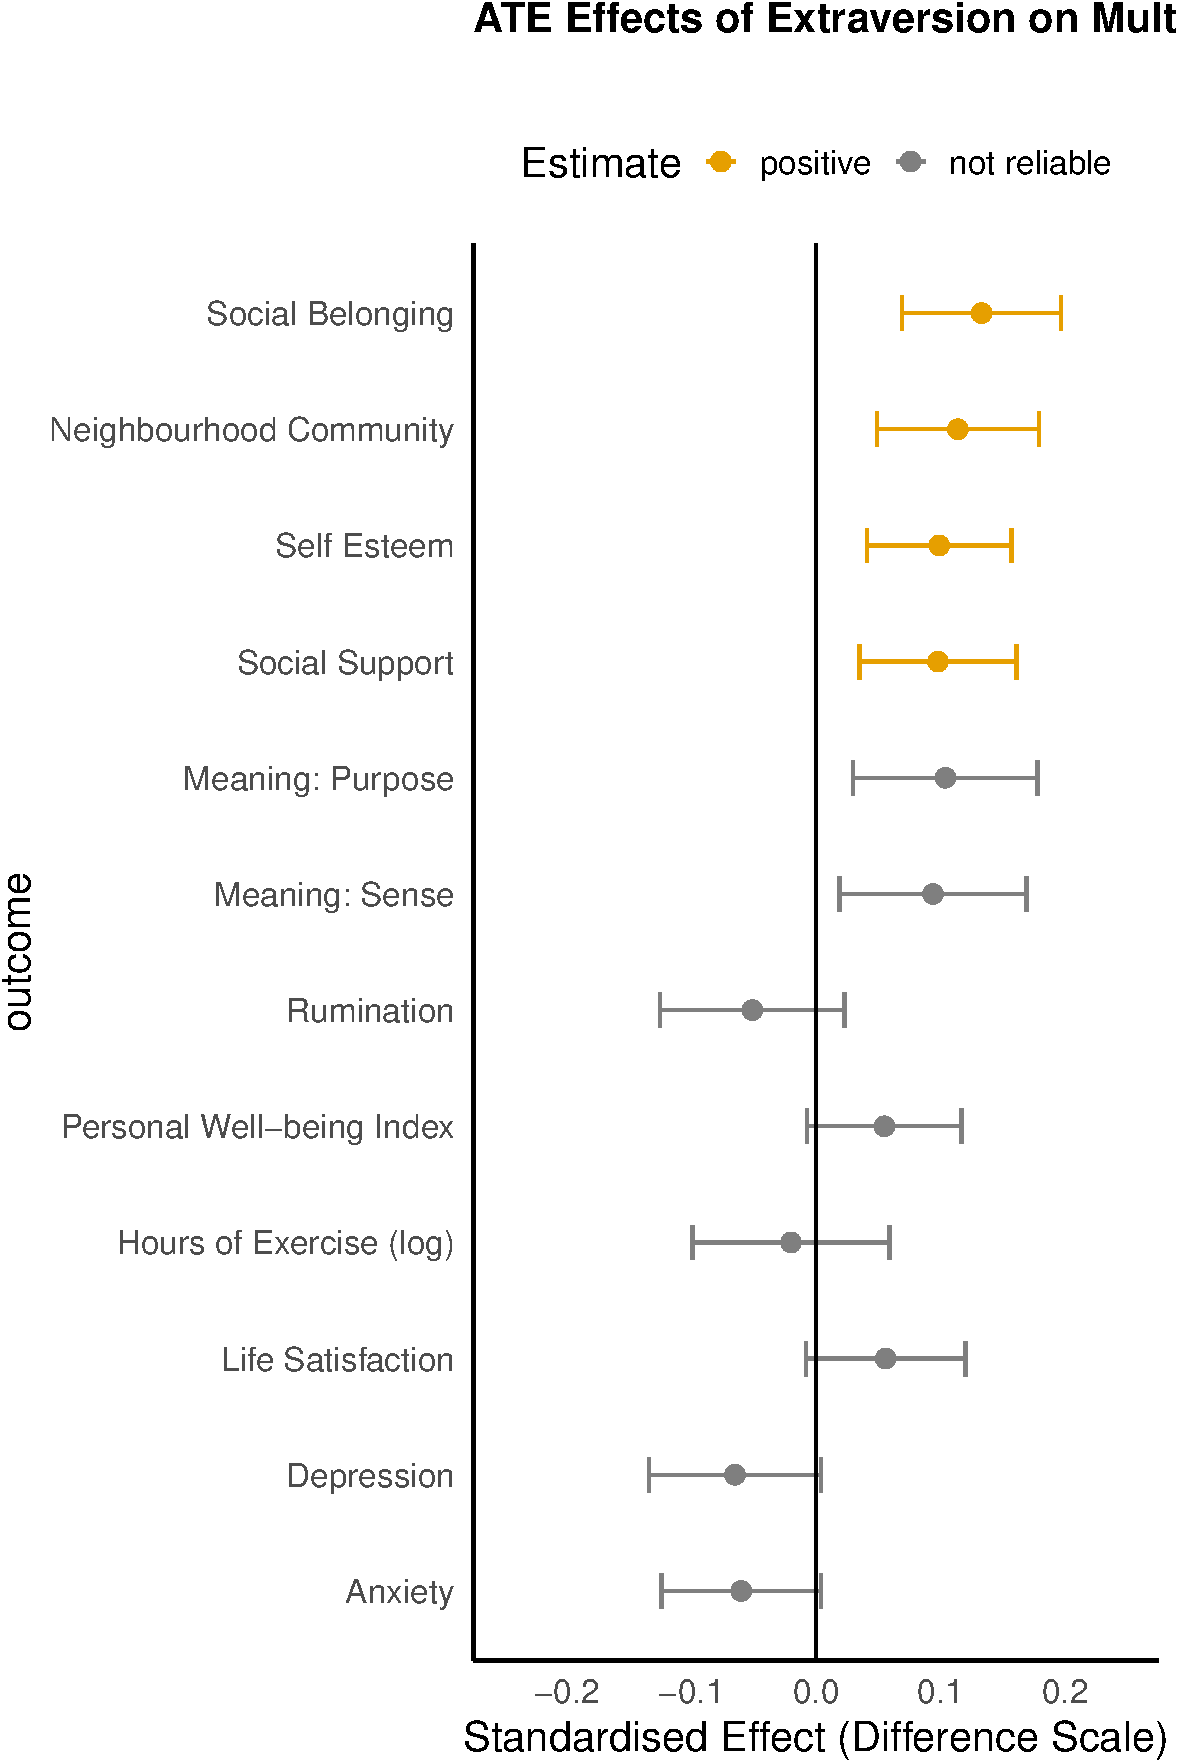
\includegraphics[keepaspectratio]{initial_quarto_document_files/figure-pdf/fig-ate-1.pdf}}

}

\caption{\label{fig-ate}Average Treatment Effects on Multi-dimensional
Wellbeing}

\end{figure}%

\newpage{}

\begin{longtable}[]{@{}
  >{\raggedright\arraybackslash}p{(\linewidth - 10\tabcolsep) * \real{0.3421}}
  >{\raggedleft\arraybackslash}p{(\linewidth - 10\tabcolsep) * \real{0.2105}}
  >{\raggedleft\arraybackslash}p{(\linewidth - 10\tabcolsep) * \real{0.0921}}
  >{\raggedleft\arraybackslash}p{(\linewidth - 10\tabcolsep) * \real{0.0921}}
  >{\raggedleft\arraybackslash}p{(\linewidth - 10\tabcolsep) * \real{0.1053}}
  >{\raggedleft\arraybackslash}p{(\linewidth - 10\tabcolsep) * \real{0.1579}}@{}}

\caption{\label{tbl-outcomes}Average Treatment Effects on
Multi-dimensional Wellbeing}

\tabularnewline

\toprule\noalign{}
\begin{minipage}[b]{\linewidth}\raggedright
\end{minipage} & \begin{minipage}[b]{\linewidth}\raggedleft
E{[}Y(1){]}-E{[}Y(0){]}
\end{minipage} & \begin{minipage}[b]{\linewidth}\raggedleft
2.5 \%
\end{minipage} & \begin{minipage}[b]{\linewidth}\raggedleft
97.5 \%
\end{minipage} & \begin{minipage}[b]{\linewidth}\raggedleft
E\_Value
\end{minipage} & \begin{minipage}[b]{\linewidth}\raggedleft
E\_Val\_bound
\end{minipage} \\
\midrule\noalign{}
\endhead
\bottomrule\noalign{}
\endlastfoot
Social Belonging & 0.128 & 0.084 & 0.171 & 1.496 & 1.375 \\
Neighbourhood Community & 0.117 & 0.071 & 0.164 & 1.466 & 1.331 \\
Social Support & 0.101 & 0.052 & 0.150 & 1.421 & 1.274 \\
Meaning: Purpose & 0.100 & 0.049 & 0.150 & 1.418 & 1.264 \\
Self Esteem & 0.089 & 0.049 & 0.129 & 1.387 & 1.260 \\
Meaning: Sense & 0.089 & 0.036 & 0.141 & 1.387 & 1.219 \\
Anxiety & -0.070 & -0.118 & -0.022 & 1.331 & 1.160 \\
Personal Well-being Index & 0.052 & 0.010 & 0.094 & 1.274 & 1.110 \\
Depression & -0.058 & -0.108 & -0.007 & 1.293 & 1.088 \\
Life Satisfaction & 0.045 & 0.000 & 0.089 & 1.250 & 1.003 \\
Rumination & -0.047 & -0.101 & 0.006 & 1.257 & 1.000 \\
Hours of Exercise (log) & -0.029 & -0.085 & 0.028 & 1.192 & 1.000 \\

\end{longtable}

The following outcomes showed reliable causal evidence (E-Value lower
bound \textgreater{} 1.2): - Social Belonging: 0.128 (0.084, 0.171); On
original scale, 0.14 (0.092, 0.187). E-Value bound = 1.375 -
Neighbourhood Community: 0.117 (0.071, 0.164); On original scale, 0.184
(0.111, 0.257). E-Value bound = 1.331 - Social Support: 0.101 (0.052,
0.15); On original scale, 0.113 (0.058, 0.168). E-Value bound = 1.274 -
Meaning: Purpose: 0.1 (0.049, 0.15); On original scale, 0.144 (0.071,
0.217). E-Value bound = 1.264 - Self Esteem: 0.089 (0.049, 0.129); On
original scale, 0.113 (0.062, 0.164). E-Value bound = 1.26 - Meaning:
Sense: 0.089 (0.036, 0.141); On original scale, 0.105 (0.043, 0.168).
E-Value bound = 1.219

\newpage{}

\subsubsection{Heterogeneous Treatment
Effects}\label{heterogeneous-treatment-effects}

\subsubsection{Comparison of targeting operating characteristic (TOC) by
rank average treatment effect (RATE): AUTOC vs
Qini}\label{comparison-of-targeting-operating-characteristic-toc-by-rank-average-treatment-effect-rate-autoc-vs-qini}

We applied two TOC by RATE methods to the same causal-forest \(\tau(x)\)
estimates:

\begin{itemize}
\item
  \textbf{AUTOC} intensifies focus on top responders via logarithmic
  weighting.
\item
  \textbf{Qini} balances effect size and prevalence via linear
  weighting.
\end{itemize}

When Qini and AUTOC disagree on positive RATE (only AUTOC yields a
positive RATE for \textbf{Hours of Exercise (log)}; only Qini yields a
positive RATE for Meaning: Sense), choose \textbf{Qini} to maximise
overall benefit or \textbf{AUTOC} to focus on top responders.

Refer to \hyperref[appendix-cate-validation]{Appendix F} for details.

\subsubsection{RATE AUTOC Results}\label{rate-autoc-results}

\subsubsection{Evidence for heterogeneous treatment effects (policy =
treat best responders) using
AUTOC}\label{evidence-for-heterogeneous-treatment-effects-policy-treat-best-responders-using-autoc}

AUTOC uses logarithmic weighting to focus treatment on top responders.

Positive RATE estimates for: \textbf{Hours of Exercise (log)}.

Estimates (\textbf{Hours of Exercise (log)}: 0.065 (95\% CI 0.014,
0.116)) show robust heterogeneity.

For outcomes with 95\%\% CI crossing zero (Meaning: Sense, Rumination,
Anxiety, Personal Well-being Index, Self Esteem, Social Belonging,
Social Support, Life Satisfaction, Meaning: Purpose, Depression,
Neighbourhood Community), evidence is inconclusive.

\begin{figure}

\centering{

\pandocbounded{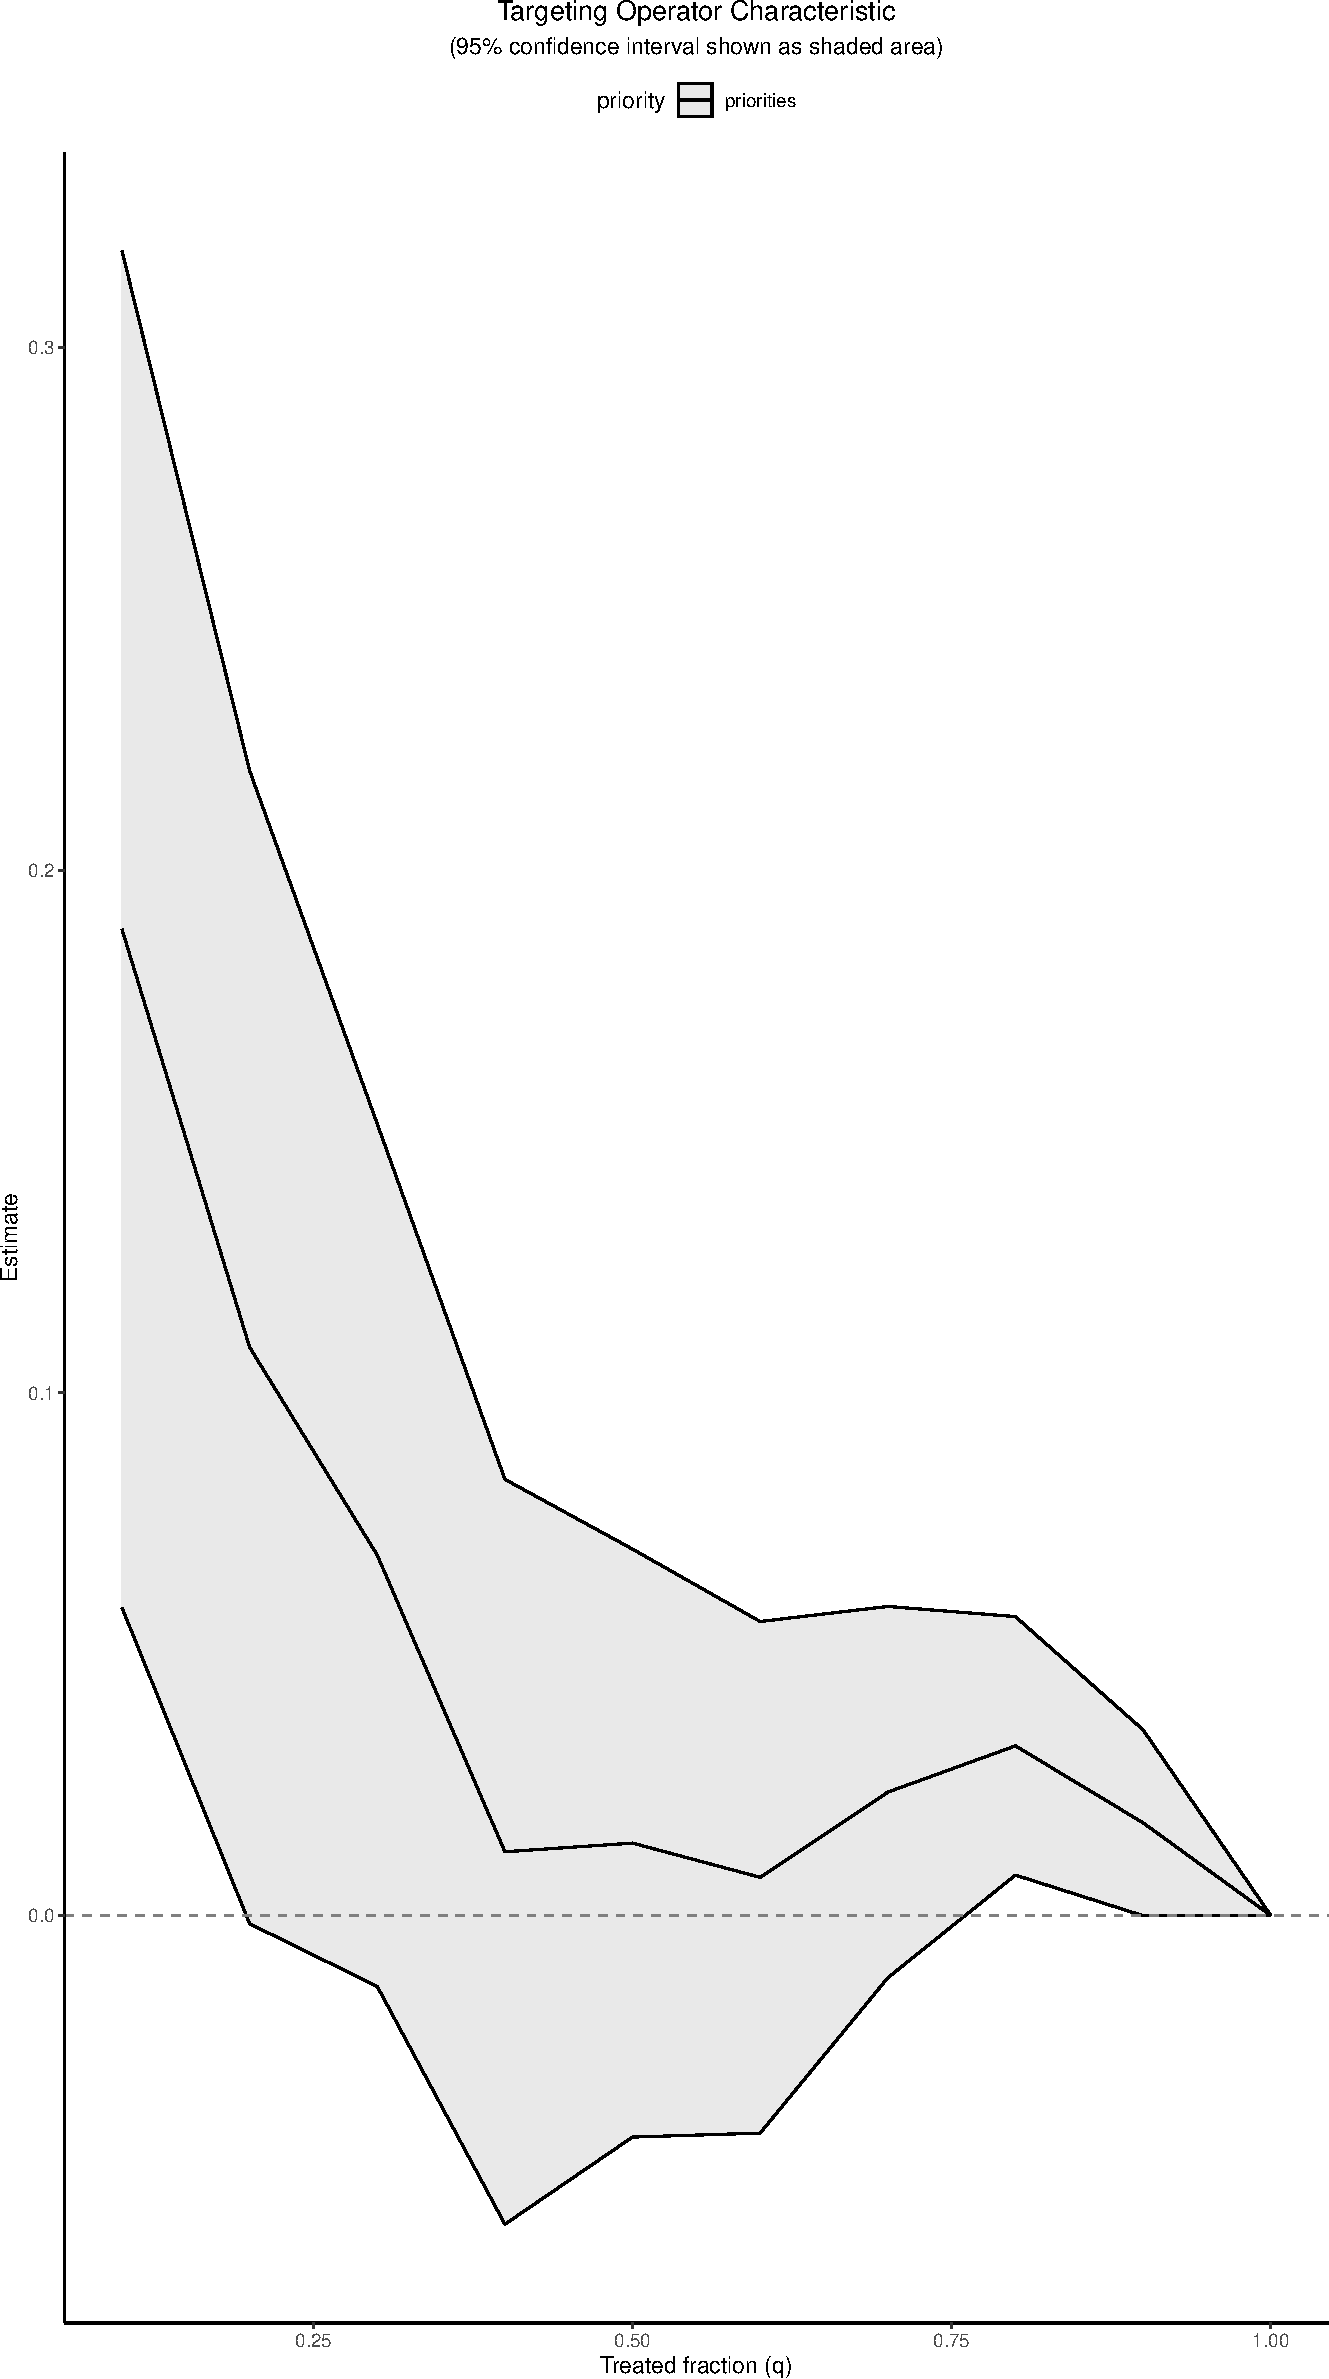
\includegraphics[keepaspectratio]{initial_quarto_document_files/figure-pdf/fig-rate-1.pdf}}

}

\caption{\label{fig-rate}RATE AUTOC Graphs}

\end{figure}%

\subsubsection{QINI Curve Results}\label{qini-curve-results}

\subsubsection{Evidence for heterogeneous treatment effects (policy =
treat best responders) using
Qini}\label{evidence-for-heterogeneous-treatment-effects-policy-treat-best-responders-using-qini}

Qini uses linear weighting to balance effect size and prevalence for
aggregate gain.

Positive RATE estimates for: \textbf{Meaning: Sense}.

Estimates (\textbf{Meaning: Sense}: 0.020 (95\% CI 0.004, 0.036)) show
robust heterogeneity.

Negative RATE estimates for: \textbf{Neighbourhood Community}.

Estimates (\textbf{Neighbourhood Community}: -0.026 (95\% CI -0.042,
-0.010)) caution against CATE prioritisation.

For outcomes with 95\%\% CI crossing zero (Hours of Exercise (log),
Personal Well-being Index, Anxiety, Self Esteem, Social Support, Life
Satisfaction, Social Belonging, Rumination, Meaning: Purpose,
Depression), evidence is inconclusive.

\begin{longtable}[]{@{}lll@{}}

\caption{\label{tbl-qini}Qini Curve Results}

\tabularnewline

\toprule\noalign{}
Model & Spend 20\% & Spend 50\% \\
\midrule\noalign{}
\endhead
\bottomrule\noalign{}
\endlastfoot
Meaning: Sense & \textbf{0.04 {[}0.01, 0.07{]}} & -0.00 {[}-0.06,
0.05{]} \\

\end{longtable}

We computed the cumulative benefits as we increase the treated fraction
by prioritising conditional average treatment effects (CATE) at two
different spend levels: 20\% of a total budget and 50\% of a total
budget, where the contrast is no priority assignment. \textbf{Meaning:
Sense} At 20\% spend: CATE prioritisation is beneficial (diff: 0.04
{[}95\% CI: 0.01, 0.07{]}). At 50 \% spend: No reliable benefits from
CATE prioritisation.

\begin{figure}

\centering{

\pandocbounded{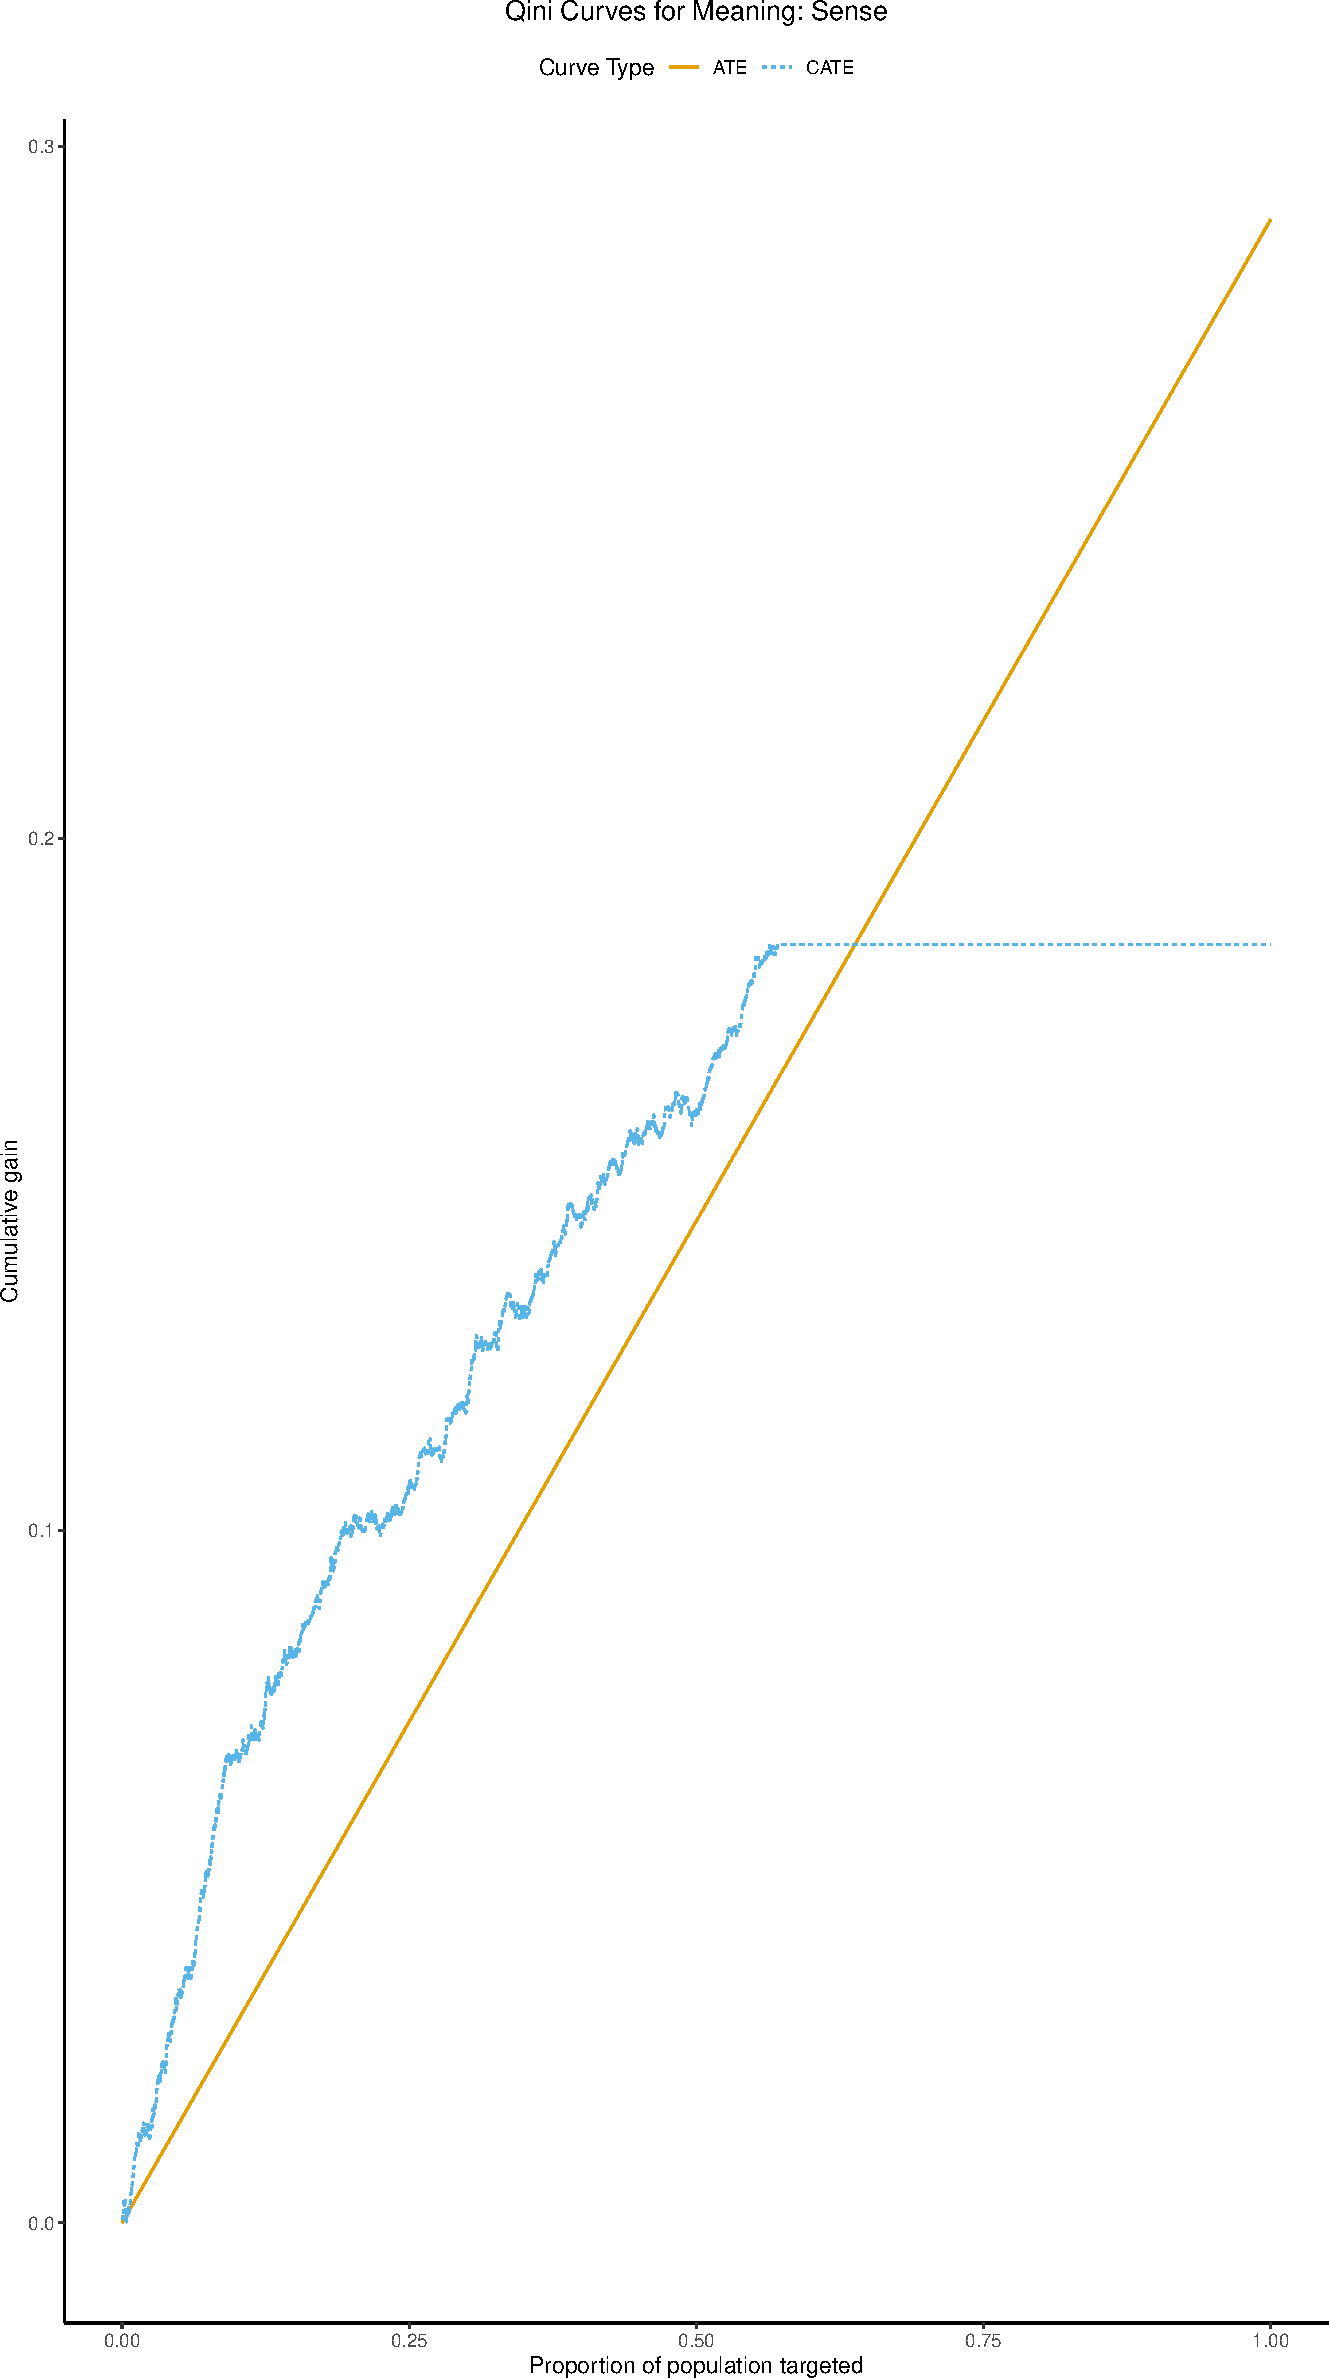
\includegraphics[keepaspectratio]{initial_quarto_document_files/figure-pdf/fig-qini-1.pdf}}

}

\caption{\label{fig-qini}RATE AUTOC Graphs}

\end{figure}%

\newpage{}

\subsubsection{Policy Trees}\label{policy-trees}

\subsubsection{Policy Tree Interpretations (depth
2)}\label{policy-tree-interpretations-depth-2}

A shallow policy tree recommends actions based on two splits for
depth=2, or one split for depth=1. We trained on 50\% of the data and
evaluated on the rest.

\textbf{Findings for log Hours Exercise:}

Split 1: Short Form Health ≤ -0.333. Within that subgroup, split 2a:
Belong ≤ -0.441, → \textbf{Control}; Belong \textgreater{} -0.441 →
\textbf{Treated}.

Split 2: Short Form Health \textgreater{} -0.333. Within that subgroup,
split 2b: Lifesat ≤ -0.268, → \textbf{Control}; Lifesat \textgreater{}
-0.268 → \textbf{Treated}.

\textbf{Findings for Meaning Sense:}

Split 1: Alcohol Intensity ≤ -0.313. Within that subgroup, split 2a: log
Hours Commute ≤ -0.496, → \textbf{Control}; log Hours Commute
\textgreater{} -0.496 → \textbf{Treated}.

Split 2: Alcohol Intensity \textgreater{} -0.313. Within that subgroup,
split 2b: Age ≤ 0.612, → \textbf{Treated}; Age \textgreater{} 0.612 →
\textbf{Control}.

\begin{figure}

\centering{

\pandocbounded{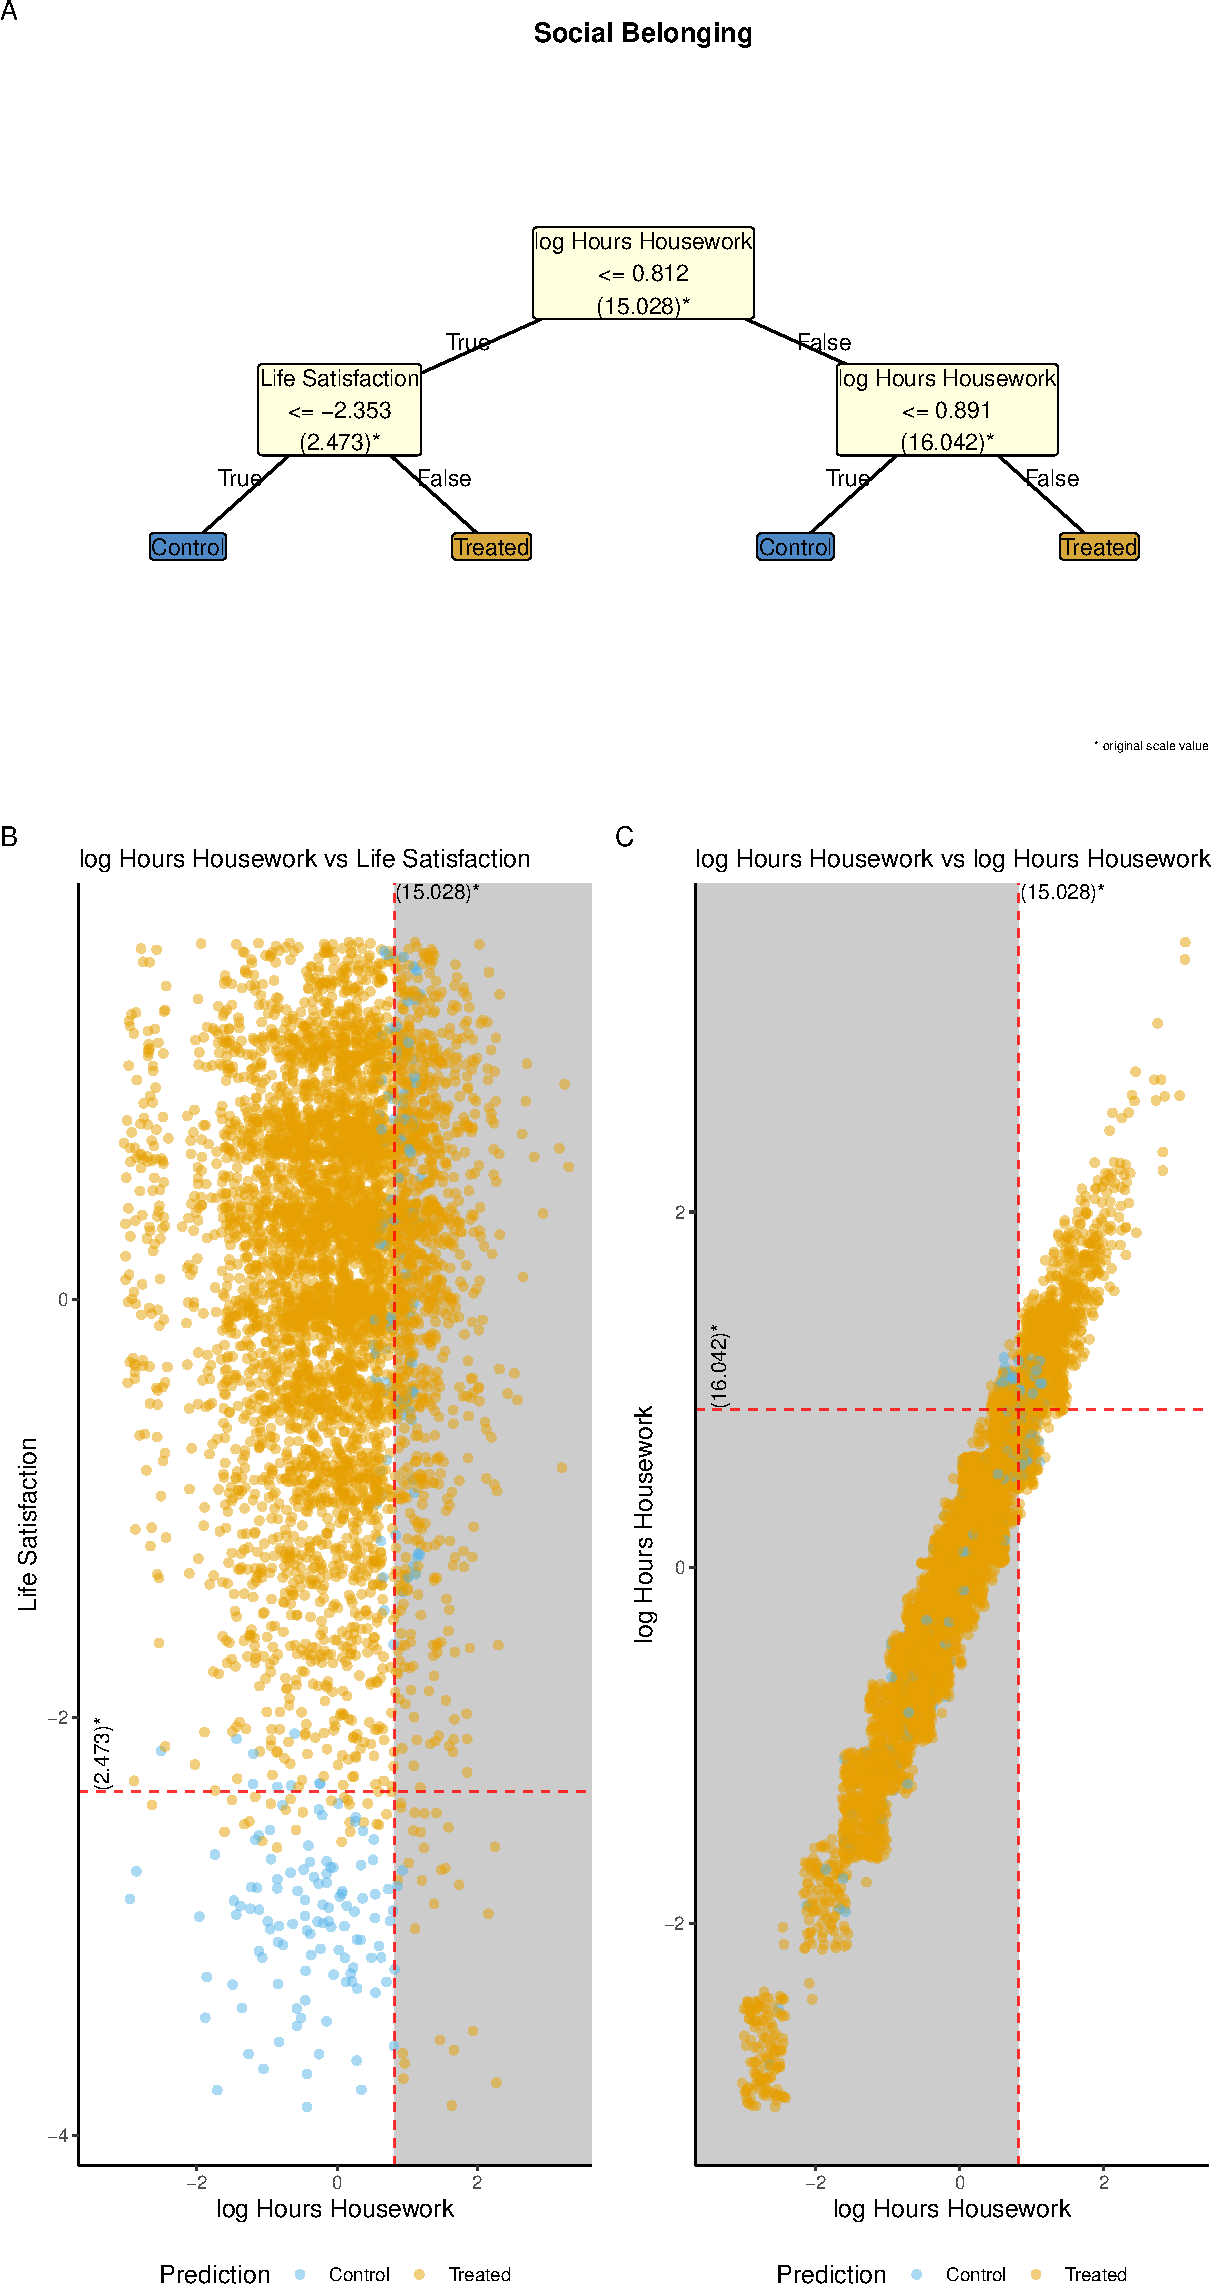
\includegraphics[keepaspectratio]{initial_quarto_document_files/figure-pdf/fig-policy-1-1.pdf}}

}

\caption{\label{fig-policy-1}Decision Tree: Exercise}

\end{figure}%

\begin{figure}

\centering{

\pandocbounded{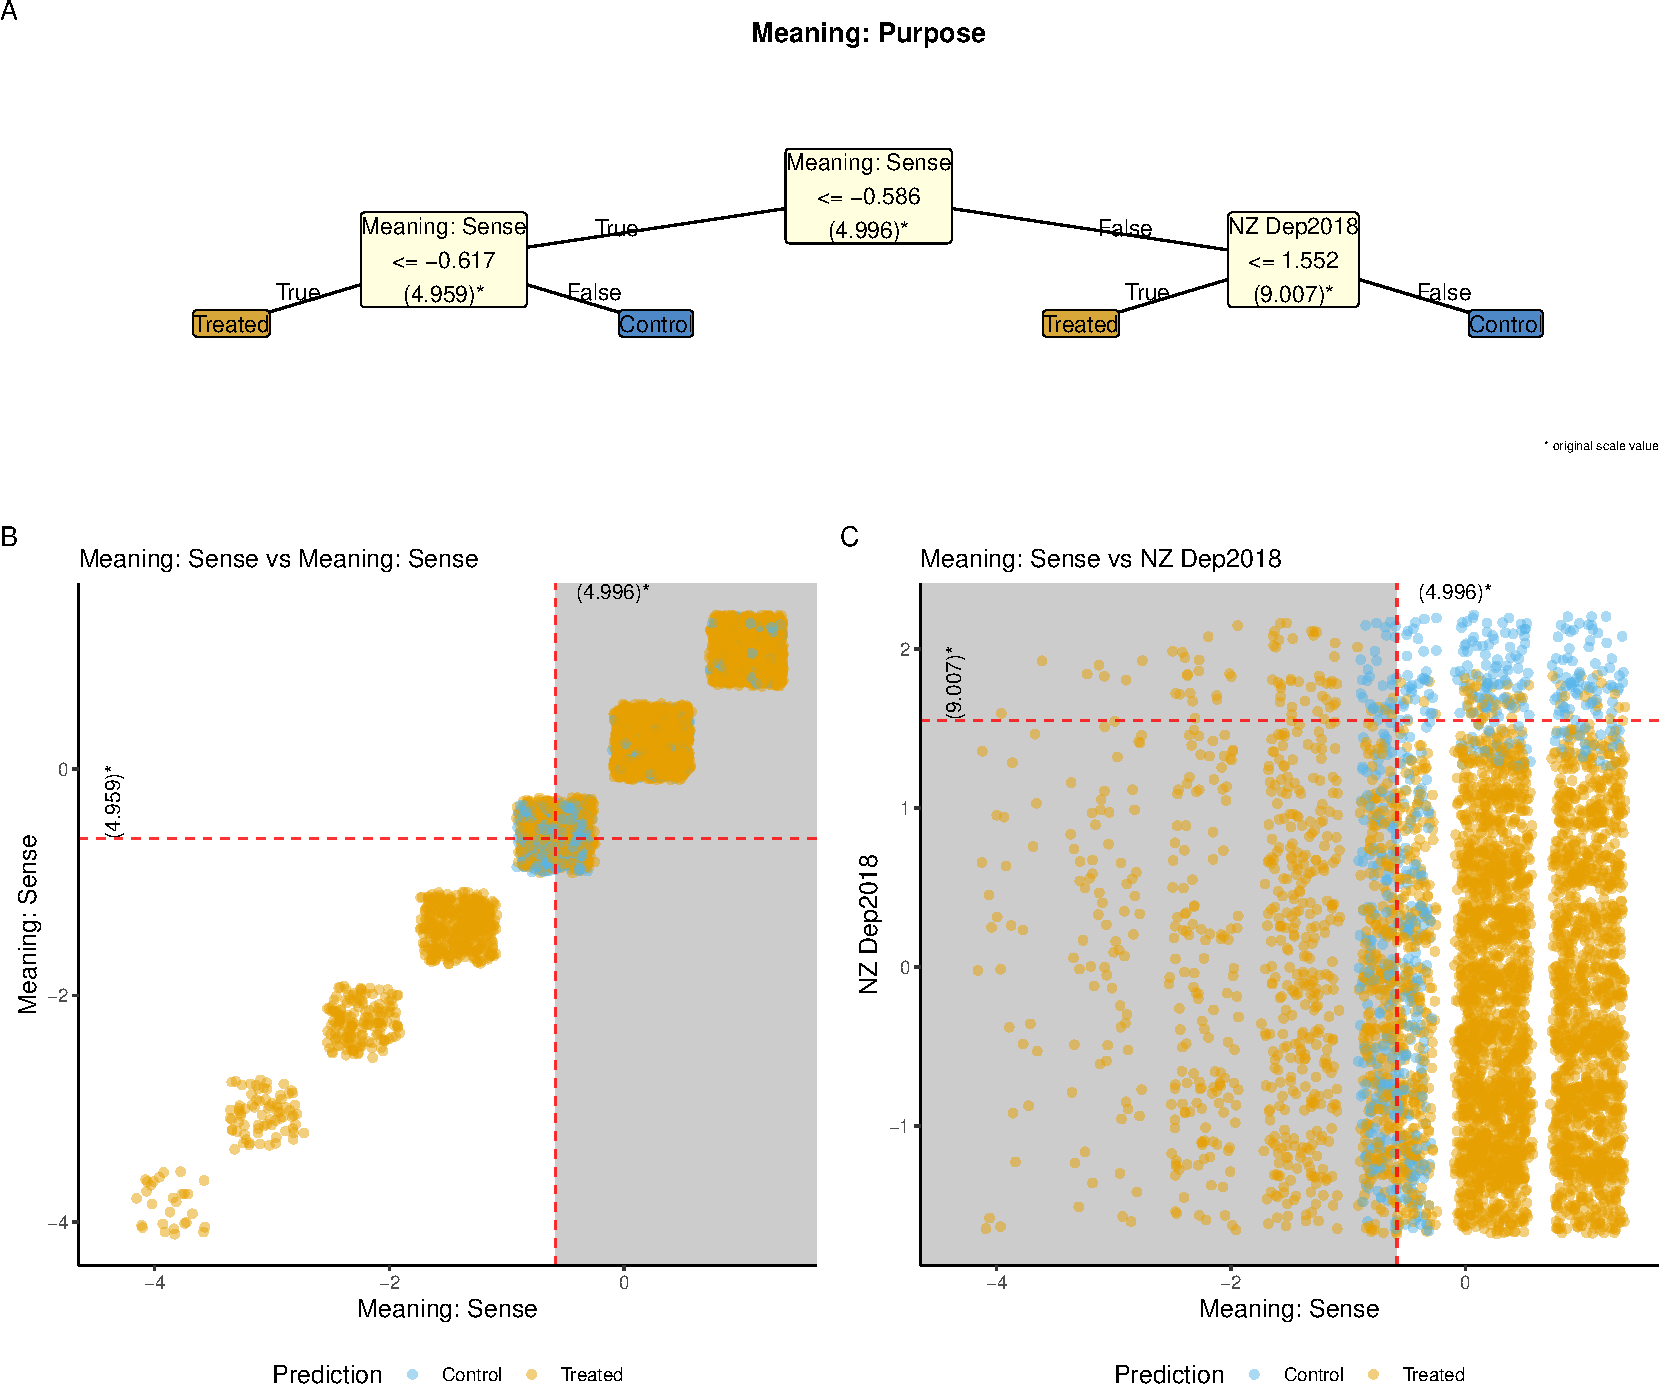
\includegraphics[keepaspectratio]{initial_quarto_document_files/figure-pdf/fig-policy-2-1.pdf}}

}

\caption{\label{fig-policy-2}Decision Tree: Meaning Sense}

\end{figure}%

\subsection{Discussion}\label{discussion}

\subsubsection{Ethics}\label{ethics}

The University of Auckland Human Participants Ethics Committee reviews
the NZAVS every three years. Our most recent ethics approval statement
is as follows: The New Zealand Attitudes and Values Study was approved
by the University of Auckland Human Participants Ethics Committee on
26/05/2021 for six years until 26/05/2027, Reference Number UAHPEC22576.

\subsubsection{Author Statement}\label{author-statement}

\subsubsection{Acknowledgements}\label{acknowledgements}

The New Zealand Attitudes and Values Study is supported by a grant from
the Templeton Religious Trust (TRT0196; TRT0418). JB received support
from the Max Plank Institute for the Science of Human History. The
funders had no role in preparing the manuscript or deciding to publish
it.

\subsubsection{Data Availability}\label{data-availability}

The data described in the paper are part of the New Zealand Attitudes
and Values Study. Members of the NZAVS management team and research
group hold full copies of the NZAVS data. A de-identified dataset
containing only the variables analysed in this manuscript is available
upon request from the corresponding author or any member of the NZAVS
advisory board for replication or checking of any published study using
NZAVS data. The code for the analysis can be found at
\href{https://osf.io/ab7cx/}{OSF link}.

\newpage{}

\subsection{Appendix A: Measures}\label{appendix-measures}

\subsubsection{Measures}\label{measures}

\paragraph{Covariate Measures}\label{covariate-measures}

\subsubsection{Baseline Covariates}\label{baseline-covariates}

\paragraph{Age}\label{age}

\emph{What is your date of birth?}

We asked participants' ages in an open-ended question (``What is your
age?'' or ``What is your date of birth'').
(\citeproc{ref-string_is}{\textbf{string\_is?}} Developed for the
NZAVS.)

\paragraph{Agreeableness}\label{agreeableness}

\emph{I sympathize with others' feelings.} \emph{I am not interested in
other people's problems.} \emph{I feel others' emotions.} \emph{I am not
really interested in others (reversed).}

Mini-IPIP6 Agreeableness dimension: (i) I sympathize with others'
feelings. (ii) I am not interested in other people's problems. (r) (iii)
I feel others' emotions. (iv) I am not really interested in others. (r)
(\citeproc{ref-sibley2011}{Sibley et al., 2011})

\paragraph{Alcohol Frequency}\label{alcohol-frequency}

\emph{``How often do you have a drink containing alcohol?''}

Participants could chose between the following responses: `(1 = Never -
I don't drink, 2 = Monthly or less, 3 = Up to 4 times a month, 4 = Up to
3 times a week, 5 = 4 or more times a week, 6 = Don't know)'
(\citeproc{ref-Ministry_of_Health_2013}{Health, 2013})

\paragraph{Alcohol Intensity}\label{alcohol-intensity}

\emph{``How many drinks containing alcohol do you have on a typical day
when drinking alcohol? (number of drinks on a typical day when
drinking)''}

Participants responded using an open-ended box.
(\citeproc{ref-Ministry_of_Health_2013}{Health, 2013})

\paragraph{Social Belonging}\label{social-belonging}

\emph{Know that people in my life accept and value me.} \emph{Feel like
an outsider (reversed).} \emph{Know that people around me share my
attitudes and beliefs.}

We assessed felt belongingness with three items adapted from the Sense
of Belonging Instrument (Hagerty \& Patusky, 1995): (1) ``Know that
people in my life accept and value me''; (2) ``Feel like an outsider'';
(3) ``Know that people around me share my attitudes and beliefs''.
Participants responded on a scale from 1 (Very Inaccurate) to 7 (Very
Accurate). The second item was reversely coded.
(\citeproc{ref-hagerty1995}{Hagerty \& Patusky, 1995})

\paragraph{Born in Nz}\label{born-in-nz}

\emph{Where were you born? (please be specific, e.g., which town/city?)}

Coded binary (1 = New Zealand; 0 = elsewhere.)
(\citeproc{ref-string_is}{\textbf{string\_is?}} Developed for the
NZAVS.)

\paragraph{Conscientiousness}\label{conscientiousness}

\emph{I get chores done right away.} \emph{I like order.} \emph{I make a
mess of things.} \emph{I often forget to put things back in their proper
place.}

Mini-IPIP6 Conscientiousness dimension: (i) I get chores done right
away. (ii) I like order. (iii) I make a mess of things. (r) (iv) I often
forget to put things back in their proper place. (r)
(\citeproc{ref-sibley2011}{Sibley et al., 2011})

\paragraph{Education Level}\label{education-level}

\emph{What is your highest level of qualification?}

We asked participants, ``What is your highest level of qualification?''.
We coded participans highest finished degree according to the New
Zealand Qualifications Authority. Ordinal-Rank 0-10 NZREG codes (with
overseas school qualifications coded as Level 3, and all other ancillary
categories coded as missing)
(\citeproc{ref-string_is}{\textbf{string\_is?}} Developed for the
NZAVS.)

\paragraph{Employed}\label{employed}

\emph{Are you currently employed (This includes self-employed of casual
work)?}

Binary response: (0 = No, 1 = Yes)
(\citeproc{ref-string_is}{\textbf{string\_is?}} Stats NZ Census
Question)

\paragraph{Ethnicity}\label{ethnicity}

\emph{Which ethnic group(s) do you belong to?}

Coded string: (1 = New Zealand European; 2 = Māori; 3 = Pacific; 4 =
Asian) (\citeproc{ref-string_is}{\textbf{string\_is?}} NZ Census
coding.)

\paragraph{Disability Status}\label{disability-status}

\emph{Do you have a health condition or disability that limits you and
that has lasted for 6+ months?}

We assessed disability with a one-item indicator adapted from Verbrugge
(1997). It asks, ``Do you have a health condition or disability that
limits you and that has lasted for 6+ months?'' (1 = Yes, 0 = No).
(\citeproc{ref-verbrugge1997}{Verbrugge, 1997})

\paragraph{Log Hours with Children}\label{log-hours-with-children}

\emph{Hours spent\ldots looking after children.}

We took the natural log of the response + 1.
(\citeproc{ref-sibley2011}{Sibley et al., 2011})

\paragraph{Log Hours Commuting}\label{log-hours-commuting}

\emph{Hours spent\ldots travelling/commuting.}

We took the natural log of the response + 1.
(\citeproc{ref-string_is}{\textbf{string\_is?}} Developed for the
NZAVS.)

\paragraph{Log Hours of Exercise}\label{log-hours-of-exercise}

\emph{Hours spent\ldots exercising/physical activity.}

We took the natural log of the response + 1.
(\citeproc{ref-sibley2011}{Sibley et al., 2011})

\paragraph{Log Hours on Housework}\label{log-hours-on-housework}

\emph{Hours spent\ldots housework/cooking.}

We took the natural log of the response + 1.
(\citeproc{ref-sibley2011}{Sibley et al., 2011})

\paragraph{Log Household Income}\label{log-household-income}

\emph{Please estimate your total household income (before tax) for the
year XXXX.}

We took the natural log of the response + 1.
(\citeproc{ref-string_is}{\textbf{string\_is?}} Developed for the
NZAVS.)

\paragraph{Male}\label{male}

\emph{We asked participants' gender in an open-ended question: ``what is
your gender?''}

Here, we coded all those who responded as Male as 1, and those who did
not as 0. (\citeproc{ref-fraser_coding_2020}{Fraser et al., 2020})

\paragraph{Neuroticism}\label{neuroticism}

\emph{I have frequent mood swings.} \emph{I am relaxed most of the time
(reversed).} \emph{I get upset easily.} \emph{I seldom feel blue
(reversed).}

Mini-IPIP6 Neuroticism dimension: (i) I have frequent mood swings. (ii)
I am relaxed most of the time. (r) (iii) I get upset easily. (iv) I
seldom feel blue. (r) (\citeproc{ref-sibley2011}{Sibley et al., 2011})

\paragraph{Non Heterosexual}\label{non-heterosexual}

\emph{How would you describe your sexual orientation? (e.g.,
heterosexual, homosexual, straight, gay, lesbian, bisexual, etc.)}

Open-ended question, coded as binary (not heterosexual = 1).
(\citeproc{ref-greaves2017diversity}{Greaves et al., 2017})

\paragraph{Nz Deprivation Index}\label{nz-deprivation-index}

\emph{New Zealand Deprivation - Decile Index - Using 2018 Census Data}

Numerical: (1-10) (\citeproc{ref-atkinson2019}{Atkinson et al., 2019})

\paragraph{Occupational Prestige
Index}\label{occupational-prestige-index}

\emph{We assessed occupational prestige and status using the New Zealand
Socio-economic Index 13 (NZSEI-13).}

This index uses the income, age, and education of a reference group, in
this case, the 2013 New Zealand census, to calculate a score for each
occupational group. Scores range from 10 (Lowest) to 90 (Highest). This
list of index scores for occupational groups was used to assign each
participant a NZSEI-13 score based on their occupation.
(\citeproc{ref-fahy2017}{Fahy et al., 2017})

\paragraph{Openness}\label{openness}

\emph{I have a vivid imagination.} \emph{I have difficulty understanding
abstract ideas (reversed).} \emph{I do not have a good imagination
(reversed).} \emph{I am not interested in abstract ideas (reversed).}

Mini-IPIP6 Openness to Experience dimension: (i) I have a vivid
imagination. (ii) I have difficulty understanding abstract ideas. (r)
(iii) I do not have a good imagination. (r) (iv) I am not interested in
abstract ideas. (r) (\citeproc{ref-sibley2011}{Sibley et al., 2011})

\paragraph{Parent}\label{parent}

\emph{If you are a parent, in which year was your eldest child born?}

Parents were coded as 1, while the others were coded as 0.
(\citeproc{ref-Developed}{\textbf{Developed?}} for the NZAVS.)

\paragraph{Has Partner}\label{has-partner}

\emph{What is your relationship status? (e.g., single, married,
de-facto, civil union, widowed, living together, etc.)}

Coded as binary (has partner = 1).
(\citeproc{ref-string_is}{\textbf{string\_is?}} Developed for the
NZAVS.)

\paragraph{Political Conservatism}\label{political-conservatism}

\emph{Please rate how politically liberal versus conservative you see
yourself as being.}

Ordinal response: (1 = Extremely Liberal, 7 = Extremely Conservative)
(\citeproc{ref-jost_end_2006-1}{Jost, 2006})

\paragraph{Religious Identification}\label{religious-identification}

\emph{How important is your religion to how you see yourself?}

Ordinal response: (1 = Not Important, 7 = Very Important)
(\citeproc{ref-string_is}{\textbf{string\_is?}} Developed for the
NZAVS.)

\paragraph{Rural Classification}\label{rural-classification}

\emph{High Urban Accessibility = 1, Medium Urban Accessibility = 2, Low
Urban Accessibility = 3, Remote = 4, Very Remote = 5.}

``Participants residence locations were coded according to a five-level
ordinal categorisation ranging from Urban to Rural.''
(\citeproc{ref-whitehead2023unmasking}{Whitehead et al., 2023})

\paragraph{Sample Frame Opt in}\label{sample-frame-opt-in}

\emph{Participant was not randomly sampled from the New Zealand
Electoral Roll.}

Code string (Binary): (0 = No, 1 = Yes)
(\citeproc{ref-string_is}{\textbf{string\_is?}} Developed for the
NZAVS.)

\paragraph{Short Form Health}\label{short-form-health}

\emph{In general, would you say your health is\ldots{}}

Ordinal response: (1 = Poor, 7 = Excellent)
(\citeproc{ref-instrument1992mos}{Instrument Ware Jr \& Sherbourne,
1992})

\paragraph{Smoker}\label{smoker}

\emph{Do you currently smoke tobacco cigarettes?}

Binary smoking indicator (0 = No, 1 = Yes).
(\citeproc{ref-string_is}{\textbf{string\_is?}} Developed for NZAVS.)

\paragraph{Exposure Measures}\label{exposure-measures}

\subsubsection{Exposure Variable}\label{exposure-variable}

\paragraph{Extraversion}\label{extraversion}

\emph{I am the life of the party.} \emph{I don't talk a lot (reversed).}
\emph{I keep in the background (reversed).} \emph{I talk to a lot of
different people at parties.}

Mini-IPIP6 Extraversion dimension: (i) I am the life of the party. (ii)
I don't talk a lot. (r) (iii) I keep in the background. (r) (iv) I talk
to a lot of different people at parties.
(\citeproc{ref-sibley2011}{Sibley et al., 2011})

\paragraph{Outcome Measures}\label{outcome-measures}

\subsubsection{Outcome Variables}\label{outcome-variables}

\paragraph{Social Belonging}\label{social-belonging-1}

\emph{Know that people in my life accept and value me.} \emph{Feel like
an outsider (reversed).} \emph{Know that people around me share my
attitudes and beliefs.}

We assessed felt belongingness with three items adapted from the Sense
of Belonging Instrument (Hagerty \& Patusky, 1995): (1) ``Know that
people in my life accept and value me''; (2) ``Feel like an outsider'';
(3) ``Know that people around me share my attitudes and beliefs''.
Participants responded on a scale from 1 (Very Inaccurate) to 7 (Very
Accurate). The second item was reversely coded.
(\citeproc{ref-hagerty1995}{Hagerty \& Patusky, 1995})

\paragraph{Anxiety}\label{anxiety}

\emph{During the past 30 days, how often did\ldots you feel restless or
fidgety?} \emph{During the past 30 days, how often did\ldots you feel
that everything was an effort?} \emph{During the past 30 days, how often
did\ldots you feel nervous?}

Ordinal response: (0 = None Of The Time; 1 = A Little Of The Time; 2=
Some Of The Time; 3 = Most Of The Time; 4 = All Of The Time)
(\citeproc{ref-kessler2002}{Kessler et al., 2002})

\paragraph{Depression}\label{depression}

\emph{During the past 30 days, how often did\ldots you feel hopeless?}
\emph{During the past 30 days, how often did\ldots you feel so depressed
that nothing could cheer you up?} \emph{During the past 30 days, how
often did\ldots you feel you feel restless or fidgety?}

Ordinal response: (0 = None Of The Time; 1 = A Little Of The Time; 2=
Some Of The Time; 3 = Most Of The Time; 4 = All Of The Time)
(\citeproc{ref-kessler2002}{Kessler et al., 2002})

\paragraph{Life Satisfaction}\label{life-satisfaction}

\emph{I am satisfied with my life.} \emph{In most ways my life is close
to ideal.}

Ordinal response (1 = Strongly Disagree to 7 = Strongly Agree).
(\citeproc{ref-diener1985a}{Diener et al., 1985})

\paragraph{Log Hours of Exercise}\label{log-hours-of-exercise-1}

\emph{Hours spent\ldots exercising/physical activity.}

We took the natural log of the response + 1.
(\citeproc{ref-sibley2011}{Sibley et al., 2011})

\paragraph{Meaning Purpose}\label{meaning-purpose}

\emph{My life has a clear sense of purpose}

Ordinal response (1 = Strongly Disagree to 7 = Strongly Agree).
(\citeproc{ref-steger_meaning_2006}{Steger et al., 2006})

\paragraph{Meaning Sense}\label{meaning-sense}

\emph{I have a good sense of what makes my life meaningful.}

Ordinal response (1 = Strongly Disagree to 7 = Strongly Agree).
(\citeproc{ref-steger_meaning_2006}{Steger et al., 2006})

\paragraph{Neighbourhood Community}\label{neighbourhood-community}

\emph{I feel a sense of community with others in my local
neighbourhood.}

Ordinal response (1 = Strongly Disagree to 7 = Strongly Agree).
(\citeproc{ref-sengupta2013}{Sengupta et al., 2013})

\paragraph{Personal Well Being Index}\label{personal-well-being-index}

no information available for this variable.

\paragraph{Rumination}\label{rumination}

\emph{During the last 30 days, how often did\ldots you have negative
thoughts that repeated over and over?}

Ordinal responses: 0 = None of The Time, 1 = A little of The Time, 2 =
Some of The Time, 3 = Most of The Time, 4 = All of The Time.
(\citeproc{ref-nolen-hoeksema_effects_1993}{Nolen-hoeksema \& Morrow,
1993})

\paragraph{Self Esteem}\label{self-esteem}

\emph{On the whole am satisfied with myself.} \emph{Take a positive
attitude toward myself.} \emph{Am inclined to feel that I am a failure
(reversed).}

Ordinal response (1 = Very inaccurate to 7 = Very accurate).
(\citeproc{ref-Rosenberg1965}{Rosenberg, 1965})

\paragraph{Social Support}\label{social-support}

\emph{There are people I can depend on to help me if I really need it.}
\emph{There is no one I can turn to for guidance in times of stress
(reversed).} \emph{I know there are people I can turn to when I need
help.}

Ordinal response: (1 = Strongly Disagree, 7 = Strongly Agree)
(\citeproc{ref-cutrona1987}{Cutrona \& Russell, 1987})

\subsection{Appendix B: Sample}\label{appendix-sample}

Table~\ref{tbl-appendix-baseline} presents sample demographic
statistics.

\begin{longtable}[]{@{}ll@{}}
\caption{Demographic statistics for New Zealand Attitudes and Values
Cohort wave 2018.}\label{tbl-appendix-baseline}\tabularnewline
\toprule\noalign{}
& 2018 \\
\midrule\noalign{}
\endfirsthead
\toprule\noalign{}
& 2018 \\
\midrule\noalign{}
\endhead
\bottomrule\noalign{}
\endlastfoot
& (N=39635) \\
\textbf{Age} & \\
Mean (SD) & 48.5 (13.9) \\
Median {[}Min, Max{]} & 51.0 {[}18.0, 99.0{]} \\
\textbf{Agreeableness} & \\
Mean (SD) & 5.35 (0.988) \\
Median {[}Min, Max{]} & 5.47 {[}1.00, 7.00{]} \\
Missing & 9 (0.0\%) \\
\textbf{Alcohol Frequency} & \\
Mean (SD) & 2.16 (1.34) \\
Median {[}Min, Max{]} & 2.00 {[}0, 5.00{]} \\
Missing & 1342 (3.4\%) \\
\textbf{Alcohol Intensity} & \\
Mean (SD) & 2.15 (2.09) \\
Median {[}Min, Max{]} & 2.00 {[}0, 15.0{]} \\
Missing & 2348 (5.9\%) \\
\textbf{Belong} & \\
Mean (SD) & 5.14 (1.07) \\
Median {[}Min, Max{]} & 5.31 {[}1.00, 7.00{]} \\
Missing & 7 (0.0\%) \\
\textbf{Born in NZ} & \\
0 & 8510 (21.5\%) \\
1 & 30670 (77.4\%) \\
Missing & 455 (1.1\%) \\
\textbf{Conscientiousness} & \\
Mean (SD) & 5.10 (1.06) \\
Median {[}Min, Max{]} & 5.23 {[}1.00, 7.00{]} \\
\textbf{Education Level} & \\
no\_qualification & 1003 (2.5\%) \\
cert\_1\_to\_4 & 13801 (34.8\%) \\
cert\_5\_to\_6 & 4953 (12.5\%) \\
university & 10400 (26.2\%) \\
post\_grad & 4220 (10.6\%) \\
masters & 3297 (8.3\%) \\
doctorate & 930 (2.3\%) \\
Missing & 1031 (2.6\%) \\
\textbf{Employed} & \\
0 & 8111 (20.5\%) \\
1 & 31475 (79.4\%) \\
Missing & 49 (0.1\%) \\
\textbf{Ethnicity} & \\
euro & 31454 (79.4\%) \\
maori & 4561 (11.5\%) \\
pacific & 971 (2.4\%) \\
asian & 2124 (5.4\%) \\
Missing & 525 (1.3\%) \\
\textbf{Disability Status} & \\
Mean (SD) & 0.223 (0.416) \\
Median {[}Min, Max{]} & 0 {[}0, 1.00{]} \\
Missing & 745 (1.9\%) \\
\textbf{Log Hours with Children} & \\
Mean (SD) & 1.18 (1.61) \\
Median {[}Min, Max{]} & 0.0341 {[}0, 5.13{]} \\
Missing & 1242 (3.1\%) \\
\textbf{Log Hours Commuting} & \\
Mean (SD) & 1.50 (0.832) \\
Median {[}Min, Max{]} & 1.61 {[}0, 4.40{]} \\
Missing & 1242 (3.1\%) \\
\textbf{Log Hours Exercising} & \\
Mean (SD) & 1.55 (0.846) \\
Median {[}Min, Max{]} & 1.61 {[}0, 4.40{]} \\
Missing & 1242 (3.1\%) \\
\textbf{Log Hours on Housework} & \\
Mean (SD) & 2.14 (0.782) \\
Median {[}Min, Max{]} & 2.20 {[}0, 5.13{]} \\
Missing & 1242 (3.1\%) \\
\textbf{Log Household Income} & \\
Mean (SD) & 11.4 (0.765) \\
Median {[}Min, Max{]} & 11.5 {[}0.685, 14.9{]} \\
Missing & 3067 (7.7\%) \\
\textbf{Male} & \\
0 & 24766 (62.5\%) \\
1 & 14767 (37.3\%) \\
Missing & 102 (0.3\%) \\
\textbf{Neuroticism} & \\
Mean (SD) & 3.49 (1.15) \\
Median {[}Min, Max{]} & 3.48 {[}1.00, 7.00{]} \\
Missing & 10 (0.0\%) \\
\textbf{Non-heterosexual} & \\
0 & 35100 (88.6\%) \\
1 & 2562 (6.5\%) \\
Missing & 1973 (5.0\%) \\
\textbf{NZ Deprivation Index} & \\
Mean (SD) & 4.77 (2.73) \\
Median {[}Min, Max{]} & 4.05 {[}1.00, 10.0{]} \\
Missing & 255 (0.6\%) \\
\textbf{Occupational Prestige Index} & \\
Mean (SD) & 54.1 (16.5) \\
Median {[}Min, Max{]} & 54.0 {[}10.0, 90.0{]} \\
Missing & 536 (1.4\%) \\
\textbf{Openness} & \\
Mean (SD) & 4.96 (1.12) \\
Median {[}Min, Max{]} & 5.00 {[}1.00, 7.00{]} \\
Missing & 3 (0.0\%) \\
\textbf{Parent} & \\
0 & 11539 (29.1\%) \\
1 & 27776 (70.1\%) \\
Missing & 320 (0.8\%) \\
\textbf{Has Partner} & \\
Mean (SD) & 0.752 (0.432) \\
Median {[}Min, Max{]} & 1.00 {[}0, 1.00{]} \\
Missing & 1244 (3.1\%) \\
\textbf{Political Conservatism} & \\
Mean (SD) & 3.59 (1.38) \\
Median {[}Min, Max{]} & 3.97 {[}1.00, 7.00{]} \\
Missing & 2682 (6.8\%) \\
\textbf{Religious Identification} & \\
Mean (SD) & 2.36 (2.18) \\
Median {[}Min, Max{]} & 1.00 {[}1.00, 7.00{]} \\
Missing & 1050 (2.6\%) \\
\textbf{Rural Classification} & \\
High Urban Accessibility & 24406 (61.6\%) \\
Medium Urban Accessibility & 7431 (18.7\%) \\
Low Urban Accessibility & 4818 (12.2\%) \\
Remote & 2241 (5.7\%) \\
Very Remote & 486 (1.2\%) \\
Missing & 253 (0.6\%) \\
\textbf{Sample Frame Opt-In} & \\
0 & 38485 (97.1\%) \\
1 & 1150 (2.9\%) \\
\textbf{Short Form Health} & \\
Mean (SD) & 5.05 (1.17) \\
Median {[}Min, Max{]} & 5.04 {[}1.00, 7.00{]} \\
Missing & 6 (0.0\%) \\
\textbf{Smoker} & \\
0 & 35771 (90.3\%) \\
1 & 2880 (7.3\%) \\
Missing & 984 (2.5\%) \\
\end{longtable}

\subsubsection{Exposure Variable}\label{appendix-exposure}

\begin{longtable}[]{@{}lll@{}}
\caption{Demographic statistics for New Zealand Attitudes and Values
Cohort waves 2018.}\label{tbl-appendix-exposures}\tabularnewline
\toprule\noalign{}
& 2018 & 2019 \\
\midrule\noalign{}
\endfirsthead
\toprule\noalign{}
& 2018 & 2019 \\
\midrule\noalign{}
\endhead
\bottomrule\noalign{}
\endlastfoot
& (N=39635) & (N=39635) \\
\textbf{Extraversion} & & \\
Mean (SD) & 3.91 (1.20) & 3.86 (1.19) \\
Median {[}Min, Max{]} & 3.96 {[}1.00, 7.00{]} & 3.79 {[}1.00, 7.00{]} \\
Missing & 0 (0\%) & 11117 (28.0\%) \\
\textbf{Extraversion (binary)} & & \\
{[}1.0,4.0{]} & 21138 (53.3\%) & 15637 (39.5\%) \\
(4.0,7.0{]} & 18497 (46.7\%) & 12881 (32.5\%) \\
Missing & 0 (0\%) & 11117 (28.0\%) \\
\end{longtable}

\newpage{}

\subsubsection{Outcome Variables}\label{appendix-outcomes}

\begin{longtable}[]{@{}
  >{\raggedright\arraybackslash}p{(\linewidth - 6\tabcolsep) * \real{0.3415}}
  >{\raggedright\arraybackslash}p{(\linewidth - 6\tabcolsep) * \real{0.2195}}
  >{\raggedright\arraybackslash}p{(\linewidth - 6\tabcolsep) * \real{0.2195}}
  >{\raggedright\arraybackslash}p{(\linewidth - 6\tabcolsep) * \real{0.2195}}@{}}
\caption{Outcome variables measured at baseline (NZAVS time 10, years
2018-2019, and time 15, years
2023-2024).}\label{tbl-appendix-outcomes}\tabularnewline
\toprule\noalign{}
\begin{minipage}[b]{\linewidth}\raggedright
\end{minipage} & \begin{minipage}[b]{\linewidth}\raggedright
2018
\end{minipage} & \begin{minipage}[b]{\linewidth}\raggedright
2020
\end{minipage} & \begin{minipage}[b]{\linewidth}\raggedright
Overall
\end{minipage} \\
\midrule\noalign{}
\endfirsthead
\toprule\noalign{}
\begin{minipage}[b]{\linewidth}\raggedright
\end{minipage} & \begin{minipage}[b]{\linewidth}\raggedright
2018
\end{minipage} & \begin{minipage}[b]{\linewidth}\raggedright
2020
\end{minipage} & \begin{minipage}[b]{\linewidth}\raggedright
Overall
\end{minipage} \\
\midrule\noalign{}
\endhead
\bottomrule\noalign{}
\endlastfoot
& (N=39635) & (N=39635) & (N=79270) \\
\textbf{Social Belonging} & & & \\
Mean (SD) & 5.14 (1.07) & 5.06 (1.09) & 5.11 (1.08) \\
Median {[}Min, Max{]} & 5.31 {[}1.00, 7.00{]} & 5.05 {[}1.00, 7.00{]} &
5.30 {[}1.00, 7.00{]} \\
Missing & 7 (0.0\%) & 13278 (33.5\%) & 13285 (16.8\%) \\
\textbf{Anxiety} & & & \\
Mean (SD) & 1.21 (0.774) & 1.17 (0.756) & 1.19 (0.767) \\
Median {[}Min, Max{]} & 1.00 {[}0, 4.00{]} & 1.00 {[}0, 4.00{]} & 1.00
{[}0, 4.00{]} \\
Missing & 51 (0.1\%) & 13275 (33.5\%) & 13326 (16.8\%) \\
\textbf{Depression} & & & \\
Mean (SD) & 0.584 (0.751) & 0.550 (0.723) & 0.571 (0.740) \\
Median {[}Min, Max{]} & 0.333 {[}0, 4.00{]} & 0.333 {[}0, 4.00{]} &
0.333 {[}0, 4.00{]} \\
Missing & 54 (0.1\%) & 13273 (33.5\%) & 13327 (16.8\%) \\
\textbf{Life Satisfaction} & & & \\
Mean (SD) & 5.30 (1.20) & 5.25 (1.23) & 5.28 (1.21) \\
Median {[}Min, Max{]} & 5.50 {[}1.00, 7.00{]} & 5.50 {[}1.00, 7.00{]} &
5.50 {[}1.00, 7.00{]} \\
Missing & 260 (0.7\%) & 13560 (34.2\%) & 13820 (17.4\%) \\
\textbf{Hours of Exercise (log)} & & & \\
Mean (SD) & 1.55 (0.846) & 1.63 (0.839) & 1.58 (0.844) \\
Median {[}Min, Max{]} & 1.61 {[}0, 4.40{]} & 1.78 {[}0, 4.40{]} & 1.61
{[}0, 4.40{]} \\
Missing & 1242 (3.1\%) & 13770 (34.7\%) & 15012 (18.9\%) \\
Meaning: Purpose & & & \\
Mean (SD) & 5.20 (1.41) & 5.15 (1.44) & 5.18 (1.42) \\
Median {[}Min, Max{]} & 5.05 {[}1.00, 7.00{]} & 5.04 {[}1.00, 7.00{]} &
5.04 {[}1.00, 7.00{]} \\
Missing & 1010 (2.5\%) & 13650 (34.4\%) & 14660 (18.5\%) \\
Meaning: Sense & & & \\
Mean (SD) & 5.71 (1.22) & 5.71 (1.19) & 5.71 (1.20) \\
Median {[}Min, Max{]} & 5.99 {[}1.00, 7.00{]} & 5.99 {[}1.00, 7.00{]} &
5.99 {[}1.00, 7.00{]} \\
Missing & 128 (0.3\%) & 13162 (33.2\%) & 13290 (16.8\%) \\
\textbf{Neighbourhood Community} & & & \\
Mean (SD) & 4.19 (1.66) & 4.38 (1.57) & 4.27 (1.63) \\
Median {[}Min, Max{]} & 4.03 {[}1.00, 7.00{]} & 4.95 {[}1.00, 7.00{]} &
4.04 {[}1.00, 7.00{]} \\
Missing & 212 (0.5\%) & 13202 (33.3\%) & 13414 (16.9\%) \\
\textbf{Pwi} & & & \\
Mean (SD) & 7.09 (1.66) & 7.18 (1.63) & 7.12 (1.65) \\
Median {[}Min, Max{]} & 7.29 {[}0, 10.0{]} & 7.47 {[}0, 10.0{]} & 7.46
{[}0, 10.0{]} \\
Missing & 41 (0.1\%) & 13120 (33.1\%) & 13161 (16.6\%) \\
\textbf{Rumination} & & & \\
Mean (SD) & 0.853 (1.00) & 0.797 (0.959) & 0.831 (0.987) \\
Median {[}Min, Max{]} & 0.955 {[}0, 4.00{]} & 0.0495 {[}0, 4.00{]} &
0.953 {[}0, 4.00{]} \\
Missing & 135 (0.3\%) & 13335 (33.6\%) & 13470 (17.0\%) \\
\textbf{Self Esteem} & & & \\
Mean (SD) & 5.14 (1.28) & 5.13 (1.27) & 5.14 (1.28) \\
Median {[}Min, Max{]} & 5.34 {[}1.00, 7.00{]} & 5.34 {[}1.00, 7.00{]} &
5.34 {[}1.00, 7.00{]} \\
Missing & 11 (0.0\%) & 13280 (33.5\%) & 13291 (16.8\%) \\
\textbf{Social Support} & & & \\
Mean (SD) & 5.95 (1.12) & 5.94 (1.12) & 5.95 (1.12) \\
Median {[}Min, Max{]} & 6.30 {[}1.00, 7.00{]} & 6.29 {[}1.00, 7.00{]} &
6.30 {[}1.00, 7.00{]} \\
Missing & 30 (0.1\%) & 13112 (33.1\%) & 13142 (16.6\%) \\
\end{longtable}

\newpage{}

\subsubsection{Appendix C: Transition Matrix to Check The Positivity
Assumption}\label{appendix-transition}

\begin{longtable}[]{@{}lrrr@{}}
\caption{Transition Matrix Showing
Change}\label{tbl-transition}\tabularnewline
\toprule\noalign{}
From / To & State 0 & State 1 & Total \\
\midrule\noalign{}
\endfirsthead
\toprule\noalign{}
From / To & State 0 & State 1 & Total \\
\midrule\noalign{}
\endhead
\bottomrule\noalign{}
\endlastfoot
State 0 & 17572 & 2271 & 19843 \\
State 1 & 2400 & 6275 & 8675 \\
\end{longtable}

These transition matrices capture shifts in states between consecutive
waves. Each cell shows the count of individuals transitioning from one
state to another. Rows are the initial state (From), columns the
subsequent state (To). \textbf{Diagonal entries} (in \textbf{bold}) mark
those who stayed in the same state.

\newpage{}

\subsection{Appendix D: Evidence of
Heterogeneity}\label{appendix-cate-validation}

\begin{longtable}[]{@{}
  >{\raggedright\arraybackslash}p{(\linewidth - 12\tabcolsep) * \real{0.2241}}
  >{\raggedright\arraybackslash}p{(\linewidth - 12\tabcolsep) * \real{0.1293}}
  >{\raggedright\arraybackslash}p{(\linewidth - 12\tabcolsep) * \real{0.1121}}
  >{\raggedright\arraybackslash}p{(\linewidth - 12\tabcolsep) * \real{0.1293}}
  >{\raggedright\arraybackslash}p{(\linewidth - 12\tabcolsep) * \real{0.1379}}
  >{\raggedright\arraybackslash}p{(\linewidth - 12\tabcolsep) * \real{0.1207}}
  >{\raggedright\arraybackslash}p{(\linewidth - 12\tabcolsep) * \real{0.1466}}@{}}
\caption{}\label{tbl-omnibus}\tabularnewline
\toprule\noalign{}
\begin{minipage}[b]{\linewidth}\raggedright
Outcome
\end{minipage} & \begin{minipage}[b]{\linewidth}\raggedright
Mean Est. (SE)
\end{minipage} & \begin{minipage}[b]{\linewidth}\raggedright
Mean p-value
\end{minipage} & \begin{minipage}[b]{\linewidth}\raggedright
Mean Status
\end{minipage} & \begin{minipage}[b]{\linewidth}\raggedright
Diff. Est. (SE)
\end{minipage} & \begin{minipage}[b]{\linewidth}\raggedright
Diff. p-value
\end{minipage} & \begin{minipage}[b]{\linewidth}\raggedright
Heterogeneity
\end{minipage} \\
\midrule\noalign{}
\endfirsthead
\toprule\noalign{}
\begin{minipage}[b]{\linewidth}\raggedright
Outcome
\end{minipage} & \begin{minipage}[b]{\linewidth}\raggedright
Mean Est. (SE)
\end{minipage} & \begin{minipage}[b]{\linewidth}\raggedright
Mean p-value
\end{minipage} & \begin{minipage}[b]{\linewidth}\raggedright
Mean Status
\end{minipage} & \begin{minipage}[b]{\linewidth}\raggedright
Diff. Est. (SE)
\end{minipage} & \begin{minipage}[b]{\linewidth}\raggedright
Diff. p-value
\end{minipage} & \begin{minipage}[b]{\linewidth}\raggedright
Heterogeneity
\end{minipage} \\
\midrule\noalign{}
\endhead
\bottomrule\noalign{}
\endlastfoot
Social Belonging & 0.98 (0.21) & 0.00e+00 & Calibrated & -1.26 (0.59) &
0.984 & No heterogeneity \\
Anxiety & 0.9 (0.47) & 0.027 & Calibrated & -1.11 (0.55) & 0.978 & No
heterogeneity \\
Depression & 1.13 (0.96) & 0.118 & Not calibrated & 0.2 (0.63) & 0.374 &
No heterogeneity \\
Life Satisfaction & 0.97 (0.44) & 0.015 & Calibrated & -0.63 (0.55) &
0.874 & No heterogeneity \\
Hours of Exercise (log) & 0.59 (1.88) & 0.377 & Not calibrated & 0.56
(0.48) & 0.121 & No heterogeneity \\
Meaning: Purpose & 0.92 (0.27) & 0.00e+00 & Calibrated & -0.35 (0.58) &
0.727 & No heterogeneity \\
Meaning: Sense & 0.95 (0.32) & 0.002 & Calibrated & 0.6 (0.42) & 0.080 &
No heterogeneity \\
Neighbourhood Community & 1 (0.2) & 0.00e+00 & Calibrated & -1.69 (0.58)
& 0.998 & No heterogeneity \\
Personal Well-being Index & 0.92 (0.36) & 0.005 & Calibrated & 0.65
(0.45) & 0.076 & No heterogeneity \\
Rumination & 0.9 (0.69) & 0.095 & Not calibrated & -0.2 (0.53) & 0.647 &
No heterogeneity \\
Self Esteem & 1.01 (0.26) & 0.00e+00 & Calibrated & 0.05 (0.52) & 0.462
& No heterogeneity \\
Social Support & 0.94 (0.29) & 0.001 & Calibrated & -0.1 (0.48) & 0.581
& No heterogeneity \\
\end{longtable}

\section{Omnibus Heterogeneity Test
Results}\label{omnibus-heterogeneity-test-results}

\subsection{Explanation}\label{explanation}

Test calibration of the forest computes the best linear fit using: 1.
Forest predictions on held-out data 2. The mean forest prediction as
regressors

Testing uses heteroskedasticity-robust (HC3) standard errors. A
coefficient of 1 for: - Mean forest prediction: indicates the mean
prediction is accurate for held-out data - Differential forest
prediction: indicates heterogeneity estimates are well calibrated

The p-value of the differential forest prediction coefficient acts as an
omnibus test for heterogeneity.

\subsection{Results by Outcome}\label{results-by-outcome}

\textbf{Social Belonging}: - Mean prediction: 0.98 (SE=0.21), t=4.71,
p=0.00e+00, calibrated. - Differential prediction: -1.26 (SE=0.59),
t=-2.15, p=0.984, no heterogeneity.

\textbf{Anxiety}: - Mean prediction: 0.9 (SE=0.47), t=1.93, p=0.027,
calibrated. - Differential prediction: -1.11 (SE=0.55), t=-2.02,
p=0.978, no heterogeneity.

\textbf{Depression}: - Mean prediction: 1.13 (SE=0.96), t=1.18, p=0.118,
not calibrated. - Differential prediction: 0.2 (SE=0.63), t=0.32,
p=0.374, no heterogeneity.

\textbf{Life Satisfaction}: - Mean prediction: 0.97 (SE=0.44), t=2.17,
p=0.015, calibrated. - Differential prediction: -0.63 (SE=0.55),
t=-1.15, p=0.874, no heterogeneity.

\textbf{Hours of Exercise (log)}: - Mean prediction: 0.59 (SE=1.88),
t=0.31, p=0.377, not calibrated. - Differential prediction: 0.56
(SE=0.48), t=1.17, p=0.121, no heterogeneity.

\textbf{Meaning: Purpose}: - Mean prediction: 0.92 (SE=0.27), t=3.43,
p=0.00e+00, calibrated. - Differential prediction: -0.35 (SE=0.58),
t=-0.6, p=0.727, no heterogeneity.

\textbf{Meaning: Sense}: - Mean prediction: 0.95 (SE=0.32), t=2.93,
p=0.002, calibrated. - Differential prediction: 0.6 (SE=0.42), t=1.41,
p=0.080, no heterogeneity.

\textbf{Neighbourhood Community}: - Mean prediction: 1 (SE=0.2), t=4.91,
p=0.00e+00, calibrated. - Differential prediction: -1.69 (SE=0.58),
t=-2.9, p=0.998, no heterogeneity.

\textbf{Personal Well-being Index}: - Mean prediction: 0.92 (SE=0.36),
t=2.57, p=0.005, calibrated. - Differential prediction: 0.65 (SE=0.45),
t=1.43, p=0.076, no heterogeneity.

\textbf{Rumination}: - Mean prediction: 0.9 (SE=0.69), t=1.31, p=0.095,
not calibrated. - Differential prediction: -0.2 (SE=0.53), t=-0.38,
p=0.647, no heterogeneity.

\textbf{Self Esteem}: - Mean prediction: 1.01 (SE=0.26), t=3.84,
p=0.00e+00, calibrated. - Differential prediction: 0.05 (SE=0.52),
t=0.1, p=0.462, no heterogeneity.

\textbf{Social Support}: - Mean prediction: 0.94 (SE=0.29), t=3.25,
p=0.001, calibrated. - Differential prediction: -0.1 (SE=0.48), t=-0.2,
p=0.581, no heterogeneity.

\subsection{Summary}\label{summary}

9 of 12 models have reliably calibrated mean predictions on held-out
data. None of the models show evidence of heterogeneity on held-out
data.

\paragraph{Rate Test}\label{rate-test}

The RATE tells us how much better we could do by offering treatment
first to those who are predicted to benefit most, rather than treating
everyone the same. A higher RATE suggests that targeting people
according to their CATE indicators can lead to `better' overall results
(where `higher' always means better, recall we flipped Anxiety,
Depression, Rumination).

\begin{longtable}[]{@{}
  >{\raggedright\arraybackslash}p{(\linewidth - 14\tabcolsep) * \real{0.3083}}
  >{\raggedright\arraybackslash}p{(\linewidth - 14\tabcolsep) * \real{0.2333}}
  >{\raggedright\arraybackslash}p{(\linewidth - 14\tabcolsep) * \real{0.0917}}
  >{\raggedright\arraybackslash}p{(\linewidth - 14\tabcolsep) * \real{0.0583}}
  >{\raggedleft\arraybackslash}p{(\linewidth - 14\tabcolsep) * \real{0.1167}}
  >{\raggedleft\arraybackslash}p{(\linewidth - 14\tabcolsep) * \real{0.0833}}
  >{\raggedleft\arraybackslash}p{(\linewidth - 14\tabcolsep) * \real{0.0583}}
  >{\raggedleft\arraybackslash}p{(\linewidth - 14\tabcolsep) * \real{0.0500}}@{}}
\caption{}\label{tbl-rate-autoc}\tabularnewline
\toprule\noalign{}
\begin{minipage}[b]{\linewidth}\raggedright
model
\end{minipage} & \begin{minipage}[b]{\linewidth}\raggedright
outcome
\end{minipage} & \begin{minipage}[b]{\linewidth}\raggedright
policy
\end{minipage} & \begin{minipage}[b]{\linewidth}\raggedright
target
\end{minipage} & \begin{minipage}[b]{\linewidth}\raggedleft
RATE Estimate
\end{minipage} & \begin{minipage}[b]{\linewidth}\raggedleft
Std Error
\end{minipage} & \begin{minipage}[b]{\linewidth}\raggedleft
2.5\%
\end{minipage} & \begin{minipage}[b]{\linewidth}\raggedleft
97.5\%
\end{minipage} \\
\midrule\noalign{}
\endfirsthead
\toprule\noalign{}
\begin{minipage}[b]{\linewidth}\raggedright
model
\end{minipage} & \begin{minipage}[b]{\linewidth}\raggedright
outcome
\end{minipage} & \begin{minipage}[b]{\linewidth}\raggedright
policy
\end{minipage} & \begin{minipage}[b]{\linewidth}\raggedright
target
\end{minipage} & \begin{minipage}[b]{\linewidth}\raggedleft
RATE Estimate
\end{minipage} & \begin{minipage}[b]{\linewidth}\raggedleft
Std Error
\end{minipage} & \begin{minipage}[b]{\linewidth}\raggedleft
2.5\%
\end{minipage} & \begin{minipage}[b]{\linewidth}\raggedleft
97.5\%
\end{minipage} \\
\midrule\noalign{}
\endhead
\bottomrule\noalign{}
\endlastfoot
model\_t2\_log\_hours\_exercise\_z & \textbf{Hours of Exercise (log)} &
treat\_best & AUTOC & 0.065 & 0.026 & 0.014 & 0.116 \\
model\_t2\_meaning\_sense\_z & Meaning: Sense & treat\_best & AUTOC &
0.061 & 0.032 & -0.002 & 0.124 \\
model\_t2\_rumination\_z & Rumination & treat\_best & AUTOC & 0.025 &
0.042 & -0.057 & 0.107 \\
model\_t2\_kessler\_latent\_anxiety\_z & Anxiety & treat\_best & AUTOC &
0.018 & 0.023 & -0.027 & 0.063 \\
model\_t2\_pwi\_z & Personal Well-being Index & treat\_best & AUTOC &
0.018 & 0.028 & -0.037 & 0.073 \\
model\_t2\_self\_esteem\_z & Self Esteem & treat\_best & AUTOC & 0.016 &
0.021 & -0.025 & 0.057 \\
model\_t2\_belong\_z & Social Belonging & treat\_best & AUTOC & -0.001 &
0.022 & -0.044 & 0.042 \\
model\_t2\_support\_z & Social Support & treat\_best & AUTOC & -0.001 &
0.038 & -0.075 & 0.073 \\
model\_t2\_lifesat\_z & Life Satisfaction & treat\_best & AUTOC & -0.013
& 0.022 & -0.056 & 0.030 \\
model\_t2\_meaning\_purpose\_z & Meaning: Purpose & treat\_best & AUTOC
& -0.031 & 0.038 & -0.105 & 0.043 \\
model\_t2\_kessler\_latent\_depression\_z & Depression & treat\_best &
AUTOC & -0.033 & 0.033 & -0.098 & 0.032 \\
model\_t2\_neighbourhood\_community\_z & Neighbourhood Community &
treat\_best & AUTOC & -0.061 & 0.039 & -0.137 & 0.015 \\
\end{longtable}

\subsubsection{Evidence for heterogeneous treatment effects (policy =
treat best responders) using
AUTOC}\label{evidence-for-heterogeneous-treatment-effects-policy-treat-best-responders-using-autoc-1}

AUTOC uses logarithmic weighting to focus treatment on top responders.

Positive RATE estimates for: \textbf{Hours of Exercise (log)}.

Estimates (\textbf{Hours of Exercise (log)}: 0.065 (95\% CI 0.014,
0.116)) show robust heterogeneity.

For outcomes with 95\%\% CI crossing zero (Meaning: Sense, Rumination,
Anxiety, Personal Well-being Index, Self Esteem, Social Belonging,
Social Support, Life Satisfaction, Meaning: Purpose, Depression,
Neighbourhood Community), evidence is inconclusive.

\begin{longtable}[]{@{}
  >{\raggedright\arraybackslash}p{(\linewidth - 14\tabcolsep) * \real{0.3058}}
  >{\raggedright\arraybackslash}p{(\linewidth - 14\tabcolsep) * \real{0.2314}}
  >{\raggedright\arraybackslash}p{(\linewidth - 14\tabcolsep) * \real{0.0909}}
  >{\raggedright\arraybackslash}p{(\linewidth - 14\tabcolsep) * \real{0.0579}}
  >{\raggedleft\arraybackslash}p{(\linewidth - 14\tabcolsep) * \real{0.1157}}
  >{\raggedleft\arraybackslash}p{(\linewidth - 14\tabcolsep) * \real{0.0826}}
  >{\raggedleft\arraybackslash}p{(\linewidth - 14\tabcolsep) * \real{0.0579}}
  >{\raggedleft\arraybackslash}p{(\linewidth - 14\tabcolsep) * \real{0.0579}}@{}}
\caption{}\label{tbl-rate-qini}\tabularnewline
\toprule\noalign{}
\begin{minipage}[b]{\linewidth}\raggedright
model
\end{minipage} & \begin{minipage}[b]{\linewidth}\raggedright
outcome
\end{minipage} & \begin{minipage}[b]{\linewidth}\raggedright
policy
\end{minipage} & \begin{minipage}[b]{\linewidth}\raggedright
target
\end{minipage} & \begin{minipage}[b]{\linewidth}\raggedleft
RATE Estimate
\end{minipage} & \begin{minipage}[b]{\linewidth}\raggedleft
Std Error
\end{minipage} & \begin{minipage}[b]{\linewidth}\raggedleft
2.5\%
\end{minipage} & \begin{minipage}[b]{\linewidth}\raggedleft
97.5\%
\end{minipage} \\
\midrule\noalign{}
\endfirsthead
\toprule\noalign{}
\begin{minipage}[b]{\linewidth}\raggedright
model
\end{minipage} & \begin{minipage}[b]{\linewidth}\raggedright
outcome
\end{minipage} & \begin{minipage}[b]{\linewidth}\raggedright
policy
\end{minipage} & \begin{minipage}[b]{\linewidth}\raggedright
target
\end{minipage} & \begin{minipage}[b]{\linewidth}\raggedleft
RATE Estimate
\end{minipage} & \begin{minipage}[b]{\linewidth}\raggedleft
Std Error
\end{minipage} & \begin{minipage}[b]{\linewidth}\raggedleft
2.5\%
\end{minipage} & \begin{minipage}[b]{\linewidth}\raggedleft
97.5\%
\end{minipage} \\
\midrule\noalign{}
\endhead
\bottomrule\noalign{}
\endlastfoot
model\_t2\_meaning\_sense\_z & \textbf{Meaning: Sense} & treat\_best &
QINI & 0.020 & 0.008 & 0.004 & 0.036 \\
model\_t2\_log\_hours\_exercise\_z & Hours of Exercise (log) &
treat\_best & QINI & 0.014 & 0.008 & -0.002 & 0.030 \\
model\_t2\_pwi\_z & Personal Well-being Index & treat\_best & QINI &
0.010 & 0.007 & -0.004 & 0.024 \\
model\_t2\_kessler\_latent\_anxiety\_z & Anxiety & treat\_best & QINI &
0.009 & 0.006 & -0.003 & 0.021 \\
model\_t2\_self\_esteem\_z & Self Esteem & treat\_best & QINI & 0.006 &
0.007 & -0.008 & 0.020 \\
model\_t2\_support\_z & Social Support & treat\_best & QINI & 0.006 &
0.008 & -0.010 & 0.022 \\
model\_t2\_lifesat\_z & Life Satisfaction & treat\_best & QINI & -0.002
& 0.006 & -0.014 & 0.010 \\
model\_t2\_belong\_z & Social Belonging & treat\_best & QINI & -0.003 &
0.007 & -0.017 & 0.011 \\
model\_t2\_rumination\_z & Rumination & treat\_best & QINI & -0.003 &
0.008 & -0.019 & 0.013 \\
model\_t2\_meaning\_purpose\_z & Meaning: Purpose & treat\_best & QINI &
-0.004 & 0.009 & -0.022 & 0.014 \\
model\_t2\_kessler\_latent\_depression\_z & Depression & treat\_best &
QINI & -0.008 & 0.007 & -0.022 & 0.006 \\
model\_t2\_neighbourhood\_community\_z & \textbf{Neighbourhood
Community} & treat\_best & QINI & -0.026 & 0.008 & -0.042 & -0.010 \\
\end{longtable}

\subsubsection{Evidence for heterogeneous treatment effects (policy =
treat best responders) using
Qini}\label{evidence-for-heterogeneous-treatment-effects-policy-treat-best-responders-using-qini-1}

Qini uses linear weighting to balance effect size and prevalence for
aggregate gain.

Positive RATE estimates for: \textbf{Meaning: Sense}.

Estimates (\textbf{Meaning: Sense}: 0.020 (95\% CI 0.004, 0.036)) show
robust heterogeneity.

Negative RATE estimates for: \textbf{Neighbourhood Community}.

Estimates (\textbf{Neighbourhood Community}: -0.026 (95\% CI -0.042,
-0.010)) caution against CATE prioritisation.

For outcomes with 95\%\% CI crossing zero (Hours of Exercise (log),
Personal Well-being Index, Anxiety, Self Esteem, Social Support, Life
Satisfaction, Social Belonging, Rumination, Meaning: Purpose,
Depression), evidence is inconclusive.

\newpage{}

\subsection*{References}\label{references}
\addcontentsline{toc}{subsection}{References}

\phantomsection\label{refs}
\begin{CSLReferences}{1}{0}
\bibitem[\citeproctext]{ref-athey2021}
Athey, S., \& Wager, S. (2021a). Policy Learning With Observational
Data. \emph{Econometrica}, \emph{89}(1), 133--161.
\url{https://doi.org/10.3982/ECTA15732}

\bibitem[\citeproctext]{ref-athey_2021_policy_tree_econometrica}
Athey, S., \& Wager, S. (2021b). Policy learning with observational
data. \emph{Econometrica}, \emph{89}(1), 133--161.
https://doi.org/\url{https://doi.org/10.3982/ECTA15732}

\bibitem[\citeproctext]{ref-atkinson2019}
Atkinson, J., Salmond, C., \& Crampton, P. (2019). \emph{NZDep2018 index
of deprivation, user{'}s manual.}

\bibitem[\citeproctext]{ref-margot2024}
Bulbulia, J. A. (2024a). \emph{Margot: MARGinal observational
treatment-effects}. \url{https://doi.org/10.5281/zenodo.10907724}

\bibitem[\citeproctext]{ref-bulbulia2024wierd}
Bulbulia, J. A. (2024b). Methods in causal inference part 3: Measurement
error and external validity threats. \emph{Evolutionary Human Sciences},
\emph{6}, e42. \url{https://doi.org/10.1017/ehs.2024.33}

\bibitem[\citeproctext]{ref-cutrona1987}
Cutrona, C. E., \& Russell, D. W. (1987). The provisions of social
relationships and adaptation to stress. \emph{Advances in Personal
Relationships}, \emph{1}, 37--67.

\bibitem[\citeproctext]{ref-diener1985a}
Diener, E., Emmons, R. A., Larsen, R. J., \& Griffin, S. (1985). The
Satisfaction With Life Scale. \emph{Journal of Personality Assessment},
\emph{49}(1), 71--75.

\bibitem[\citeproctext]{ref-fahy2017}
Fahy, K. M., Lee, A., \& Milne, B. J. (2017). \emph{{N}ew {Z}ealand
socio-economic index 2013}. Statistics New Zealand-Tatauranga Aotearoa.

\bibitem[\citeproctext]{ref-fraser_coding_2020}
Fraser, G., Bulbulia, J., Greaves, L. M., Wilson, M. S., \& Sibley, C.
G. (2020). Coding responses to an open-ended gender measure in a {N}ew
{Z}ealand national sample. \emph{The Journal of Sex Research},
\emph{57}(8), 979--986.
\url{https://doi.org/10.1080/00224499.2019.1687640}

\bibitem[\citeproctext]{ref-greaves2017diversity}
Greaves, L. M., Barlow, F. K., Lee, C. H., Matika, C. M., Wang, W.,
Lindsay, C.-J., Case, C. J., Sengupta, N. K., Huang, Y., Cowie, L. J.,
et al. (2017). The diversity and prevalence of sexual orientation
self-labels in a {N}ew {Z}ealand national sample. \emph{Archives of
Sexual Behavior}, \emph{46}, 1325--1336.

\bibitem[\citeproctext]{ref-hagerty1995}
Hagerty, B. M. K., \& Patusky, K. (1995). Developing a Measure Of Sense
of Belonging: \emph{Nursing Research}, \emph{44}(1), 9--13.
\url{https://doi.org/10.1097/00006199-199501000-00003}

\bibitem[\citeproctext]{ref-Ministry_of_Health_2013}
Health, Ministry of. (2013). \emph{The {N}ew {Z}ealand {H}ealth
{S}urvey: Content guide 2012-2013}. Princeton University Press.

\bibitem[\citeproctext]{ref-hernan2016}
Hernán, M. A., Sauer, B. C., Hernández-Díaz, S., Platt, R., \& Shrier,
I. (2016). Specifying a target trial prevents immortal time bias and
other self-inflicted injuries in observational analyses. \emph{Journal
of Clinical Epidemiology}, \emph{79}, 70--75.

\bibitem[\citeproctext]{ref-instrument1992mos}
Instrument Ware Jr, J., \& Sherbourne, C. (1992). The MOS 36-item
short-form health survey (SF-36): I. Conceptual framework and item
selection. \emph{Medical Care}, \emph{30}(6), 473--483.

\bibitem[\citeproctext]{ref-jost_end_2006-1}
Jost, J. T. (2006). The end of the end of ideology. \emph{American
Psychologist}, \emph{61}(7), 651--670.
\url{https://doi.org/10.1037/0003-066X.61.7.651}

\bibitem[\citeproctext]{ref-kessler2002}
Kessler, R. ~C., Andrews, G., Colpe, L. ~J., Hiripi, E., Mroczek, D.
~K., Normand, S.-L. ~T., Walters, E. ~E., \& Zaslavsky, A. ~M. (2002).
Short screening scales to monitor population prevalences and trends in
non-specific psychological distress. \emph{Psychological Medicine},
\emph{32}(6), 959--976. \url{https://doi.org/10.1017/S0033291702006074}

\bibitem[\citeproctext]{ref-linden2020EVALUE}
Linden, A., Mathur, M. B., \& VanderWeele, T. J. (2020). Conducting
sensitivity analysis for unmeasured confounding in observational studies
using e-values: The evalue package. \emph{The Stata Journal},
\emph{20}(1), 162--175.

\bibitem[\citeproctext]{ref-nolen-hoeksema_effects_1993}
Nolen-hoeksema, S., \& Morrow, J. (1993). Effects of rumination and
distraction on naturally occurring depressed mood. \emph{Cognition and
Emotion}, \emph{7}(6), 561--570.
\url{https://doi.org/10.1080/02699939308409206}

\bibitem[\citeproctext]{ref-pearl2009a}
Pearl, J. (2009). \emph{Causality}. Cambridge University Press.

\bibitem[\citeproctext]{ref-Rosenberg1965}
Rosenberg, M. (1965). \emph{Society and the adolescent self-image}.
Princeton University Press.

\bibitem[\citeproctext]{ref-sengupta2013}
Sengupta, N. K., Luyten, N., Greaves, L. M., Osborne, D., Robertson, A.,
Brunton, C., Armstrong, G., \& Sibley, C. G. (2013). Sense of Community
in {N}ew {Z}ealand Neighbourhoods: A Multi-Level Model Predicting Social
Capital. \emph{New Zealand Journal of Psychology}, \emph{42}(1), 36--45.

\bibitem[\citeproctext]{ref-sibley2021}
Sibley, C. G. (2021). \emph{Sampling procedure and sample details for
the {N}ew {Z}ealand {A}ttitudes and {V}alues {S}tudy}.
\url{https://doi.org/10.31234/osf.io/wgqvy}

\bibitem[\citeproctext]{ref-sibley2011}
Sibley, C. G., Luyten, N., Purnomo, M., Mobberley, A., Wootton, L. W.,
Hammond, M. D., Sengupta, N., Perry, R., West-Newman, T., Wilson, M. S.,
McLellan, L., Hoverd, W. J., \& Robertson, A. (2011). The Mini-IPIP6:
Validation and extension of a short measure of the Big-Six factors of
personality in {N}ew {Z}ealand. \emph{New Zealand Journal of
Psychology}, \emph{40}(3), 142--159.

\bibitem[\citeproctext]{ref-steger_meaning_2006}
Steger, M. F., Frazier, P., Oishi, S., \& Kaler, M. (2006). The meaning
in life questionnaire: Assessing the presence of and search for meaning
in life. \emph{Journal of Counseling Psychology}, \emph{53}(1), 80--93.
\url{https://doi.org/10.1037/0022-0167.53.1.80}

\bibitem[\citeproctext]{ref-policytree_package_2024}
Sverdrup, E., Kanodia, A., Zhou, Z., Athey, S., \& Wager, S. (2024).
\emph{Policytree: Policy learning via doubly robust empirical welfare
maximization over trees}.
\url{https://CRAN.R-project.org/package=policytree}

\bibitem[\citeproctext]{ref-grf2024}
Tibshirani, J., Athey, S., Sverdrup, E., \& Wager, S. (2024). \emph{Grf:
Generalized random forests}. \url{https://github.com/grf-labs/grf}

\bibitem[\citeproctext]{ref-vanderweele2019}
VanderWeele, T. J. (2019). Principles of confounder selection.
\emph{European Journal of Epidemiology}, \emph{34}(3), 211--219.

\bibitem[\citeproctext]{ref-vanderweele2017}
VanderWeele, T. J., \& Ding, P. (2017). Sensitivity analysis in
observational research: Introducing the {E}-value. \emph{Annals of
Internal Medicine}, \emph{167}(4), 268--274.
\url{https://doi.org/10.7326/M16-2607}

\bibitem[\citeproctext]{ref-vanderweele2020}
VanderWeele, T. J., Mathur, M. B., \& Chen, Y. (2020). Outcome-wide
longitudinal designs for causal inference: A new template for empirical
studies. \emph{Statistical Science}, \emph{35}(3), 437--466.

\bibitem[\citeproctext]{ref-verbrugge1997}
Verbrugge, L. M. (1997). A global disability indicator. \emph{Journal of
Aging Studies}, \emph{11}(4), 337--362.
\url{https://doi.org/10.1016/S0890-4065(97)90026-8}

\bibitem[\citeproctext]{ref-wager2018}
Wager, S., \& Athey, S. (2018). Estimation and inference of
heterogeneous treatment effects using random forests. \emph{Journal of
the American Statistical Association}, \emph{113}(523), 1228--1242.
\url{https://doi.org/10.1080/01621459.2017.1319839}

\bibitem[\citeproctext]{ref-whitehead2023unmasking}
Whitehead, J., Davie, G., Graaf, B. de, Crengle, S., Lawrenson, R.,
Miller, R., \& Nixon, G. (2023). Unmasking hidden disparities: A
comparative observational study examining the impact of different
rurality classifications for health research in aotearoa new zealand.
\emph{BMJ Open}, \emph{13}(4), e067927.

\end{CSLReferences}




\end{document}
